\documentclass[a4paper,fleqn]{cas-dc}
\usepackage[authoryear,longnamesfirst]{natbib}
\usepackage{amsmath,amssymb,amsfonts}
\usepackage{graphicx}
\usepackage{booktabs}
\usepackage{multirow}
\usepackage{array}
\usepackage{xcolor}
\usepackage{algorithm}
\usepackage{algorithmic}
\usepackage{url}
\usepackage{lineno}

\graphicspath{{./}}

%% ─── Running headers ─────────────────────────────────────────────────────────
\shorttitle{FMBM-Net: Federated Multi-Scale Bio-Multimodal Network}
\shortauthors{S. Tanala}

\begin{document}

\let\WriteBookmarks\relax
\def\floatpagepagefraction{1}
\def\textpagefraction{.001}

%% ─── Title ───────────────────────────────────────────────────────────────────
\title[mode=title]{FMBM-Net: A Federated Multi-Scale Bio-Multimodal Network
with Latent Cross-Attention Transformer for Privacy-Preserving Biomedical AI}

\tnotemark[1]
\tnotetext[1]{This work was supported in part by ANITS Seed Research Grant
No.~ANITS/SRG/2025-26/EEE-04. Code, pre-processed splits, and training scripts
are publicly available at
\url{https://github.com/subrahmanyamtanala-rgb/fmbm-net}.}

%% ─── Author ──────────────────────────────────────────────────────────────────
\author[1]{Subrahmanyam Tanala}[
  role=Corresponding Author,
  orcid=0000-0002-4891-3122]
\cormark[1]
\fnmark[1]
\ead{tanala.subrahmanyam@anits.edu.in}
\credit{Conceptualization, Methodology, Software, Formal Analysis,
        Writing -- Original Draft, Writing -- Review \& Editing}

\affiliation[1]{organization={Department of Electrical and Electronics
Engineering, Anil Neerukonda Institute of Technology and Sciences (ANITS)},
  addressline={Sangivalasa},
  city={Visakhapatnam},
  postcode={531162},
  state={Andhra Pradesh},
  country={India}}

\cortext[cor1]{Corresponding author}
\fntext[fn1]{Manuscript submitted May 2026.}

%% ─── Abstract ────────────────────────────────────────────────────────────────
\begin{highlights}
\item FMBM-Net federates genomic, imaging, and EHR modalities under a single $(\varepsilon,\delta)$-DP pipeline.
\item The novel FLCAT performs cross-modal attention in differentially-private latent space without raw data sharing.
\item Boundary-guided Region Uncertainty Estimation (RUE) suppresses noisy CT/MRI annotation effects during FL.
\item 10-seed bootstrap evaluation across four public benchmarks; all gains statistically significant ($p<0.01$).
\item Risk-Stratified Governance Controller (RSGC) generates regulatory-aligned audit trails at inference time.
\end{highlights}

\begin{abstract}
The convergence of genomic sequences, three-dimensional volumetric medical
images, and longitudinal electronic health records~(EHR) represents a paradigm
shift in precision medicine. Yet two fundamental barriers persist: patient data
cannot be centrally aggregated without violating stringent privacy regulations,
and no existing federated learning~(FL) framework provides principled
cross-modal fusion across all three modalities simultaneously. This paper
introduces the Federated Multi-Scale Bio-Multimodal Network (FMBM-Net),
a novel architecture that resolves both challenges through three synergistic
modules. First, the Federated Latent Cross-Attention Transformer
(FLCAT) performs $H$-head cross-modal attention with complete residual
connections and layer normalization entirely within a
$(\varepsilon,\delta)$-differentially private latent space, enabling
genome$\leftrightarrow$imaging$\leftrightarrow$EHR reasoning without
transmitting raw patient data. Second, a boundary-guided Region
Uncertainty Estimation~(RUE) module applies Monte Carlo dropout-based per-voxel confidence scoring to suppress the effect of noisy CT/MRI annotations during federated training. Third, a deterministic Risk-Stratified Governance Controller~(RSGC) with a four-tier confidence finite-state machine is \emph{designed to align with} emerging healthcare AI regulatory frameworks, including the EU AI Act and updated HIPAA guidance. Comprehensive evaluation on four real public benchmarks---CADD~v1.7 ($n\!=\!35{,}000$ variants), MSD Pancreas-CT ($n\!=\!281$ volumes), MIMIC-IV~v2.2 ($n\!=\!52{,}143$ admissions), and a curated TCGA-LUNG multimodal cohort ($n\!=\!1{,}000$ patients)---using 10 independent random seeds and bootstrap 95\,\% confidence intervals demonstrates that FMBM-Net achieves multimodal AUROC $0.947\!\pm\!0.007$, CT Dice $0.934\!\pm\!0.011$, GradCAM++ IoU $0.634\!\pm\!0.029$, and expert-agreement $0.76\!\pm\!0.03$ at privacy budget $\varepsilon\!=\!2.0$, $\delta\!=\!10^{-5}$. All improvements over the best federated baseline (MOON) are statistically significant (Wilcoxon signed-rank test, $p\!<\!0.01$; Cohen's $d\!\geq\!1.2$).
\end{abstract}

\begin{keywords}
Federated learning \sep
Multimodal biomedical AI \sep
Cross-attention transformer \sep
Differential privacy \sep
Genomic modeling \sep
Medical image segmentation \sep
Electronic health records \sep
Explainable AI \sep
Regulatory compliance \sep
Precision medicine
\end{keywords}

\maketitle

%% =============================================================================
\section{Introduction}
\label{sec:intro}
%% =============================================================================

The vision of precision medicine---tailoring clinical decisions to an individual's molecular, anatomical, and longitudinal health profile---demands the simultaneous integration of genomic sequences, three-dimensional~(3D) volumetric medical images, and electronic health records~(EHR). Each modality encodes complementary biological signal: genomic variants encode susceptibility and therapeutic target information; volumetric imaging captures macro-scale structural and textural phenotypes; and longitudinal EHR streams encode  treatment trajectories and comorbidity patterns. Realizing this vision in clinical practice faces two fundamental obstacles.

\textbf{Privacy and regulatory barriers.} Centralizing multi-modal patient data across institutions is prohibited under major healthcare regulatory frameworks, including HIPAA~\citep{hipaa_guidance_2024} and the EU AI
Act~\citep{eu_ai_act_2024}. Federated learning~(FL) offers a principled solution: models are trained across distributed clinical sites without raw data leaving the local node. Yet existing FL frameworks---FedAvg~\citep{mcmahan2017}, FedProx~\citep{li2020fedprox}, MOON~\citep{li2021moon}---treat each modality as an independent silo and offer no mechanism for cross-modal fusion in the federated setting.

\textbf{Annotation noise and multi-modal alignment.} Medical imaging labels are frequently noisy owing to inter-annotator disagreement, particularly at tissue boundaries in CT and MRI scans \citep{rue_ct_2025}. Standard federated models propagate this label noise into the global model, inflating boundary-region variance. Moreover, aligning heterogeneous latent representations from
genomic sequences (discrete tokens), volumetric images (dense voxel grids), and EHR time series (irregular multivariate signals) within a single differentially private pipeline remains an unsolved problem.

In this paper, we introduce \textbf{FMBM-Net}, which, to our knowledge, is among the first federated architectures to natively unify genomic, imaging, and EHR modalities under a single $(\varepsilon,\delta)$-DP pipeline. The architecture is illustrated in Fig.~\ref{fig:arch}.

\textbf{Summary of contributions:}
\begin{enumerate}
\item \textbf{FMBM-Net}: a federated three-modality architecture that processes
  genomic sequences via an Evo~2-inspired Genomic Expert Network~(GEN)
  \citep{evo2_2026}, volumetric images via a noise-aware 3D encoder, and EHR
  via a DenseFormer-MoE \citep{denseformer2024}, all within a single
  $(\varepsilon,\delta)$-DP federated pipeline.

\item \textbf{FLCAT}: a fully-specified Federated Latent Cross-Attention
  Transformer with complete $Q/K/V$ projections, multi-head aggregation,
  residual connections, and LayerNorm, operating in differentially-private
  latent space. The FLCAT adds only $0.48$~GFLOPs and exhibits
  $O(M^2 d_k)$ complexity with $M\!=\!3$ modalities.

\item \textbf{RUE module}: boundary-guided per-voxel confidence scoring via Monte Carlo dropout ($K\!=\!10$ passes) with a noise-aware training loss, reducing CT Dice variance by $30\,\%$ relative to standard nnU-Net.

\item \textbf{RSGC}: a deterministic four-tier confidence finite-state machine
  generating regulatory compliance audit trails, \emph{designed to align with} the BMJ risk-stratified framework \citep{bmj_governance_2026} and EU AIAct \citep{eu_ai_act_2024}.

\item \textbf{Rigorous evaluation}: 10-seed bootstrap confidence intervals, Cohen's $d$ effect sizes, Wilcoxon signed-rank tests, Dirichlet heterogeneity sweeps, client dropout robustness experiments, and quantitative XAI metrics on four real public benchmarks.
\end{enumerate}

The manuscript is organized as follows.
Section~\ref{sec:related} reviews related work.
Section~\ref{sec:architecture} describes FMBM-Net in full.
Section~\ref{sec:training} details the training procedure.
Section~\ref{sec:experiments} reports experimental results.
Section~\ref{sec:discussion} provides extended discussion.
Section~\ref{sec:conclusion} concludes.

\subsection{Motivating Clinical Scenario}

To ground the contributions in clinical reality, consider a representative use case: a 58-year-old patient presents with an incidental pulmonary nodule detected on a routine chest CT. Optimal management requires integrating
(i)~germline/somatic mutation data from a liquid biopsy
(KRAS~G12C and STK11 co-mutation patterns),
(ii)~volumetric radiomic features from the 3D CT, and
(iii)~longitudinal clinical history including smoking status, medication
exposures, and prior oncology encounters in the EHR. Individually, imaging alone yields a malignancy probability of $\sim$60\,\%. Integrated multimodal assessment shifts this to $\sim$89\,\%, directly influencing whether the clinical recommendation is surveillance or biopsy. Yet in practice, genomic data resides at a molecular pathology laboratory, imaging at a radiology PACS, and EHR data at a clinical information system---often across separate
institutions and jurisdictions. FMBM-Net is specifically designed to enable this trimodal reasoning without any data source crossing institutional boundaries.

\subsection{Scope and Assumptions}

FMBM-Net targets the setting where $C$ clinical sites each hold all three modalities for their local patient populations, and a trusted aggregation server coordinates training without accessing raw data. We assume:
(i)~honest-but-curious participants; (ii)~synchronous communication in
Phase~2; and (iii)~a jointly agreed-upon $(\varepsilon,\delta)$ budget.
Asynchronous, Byzantine-robust, and adaptive-budget extensions are deferred
to future work.

\subsection{Motivating Clinical Scenario}

To ground the abstract technical contributions in clinical reality, consider the following representative use case. A 58-year-old patient presents with an incidental pulmonary nodule detected on a routine chest CT scan. Optimal management depends on integrating three information streams: (i)~germline and
somatic mutation data from a liquid biopsy identifying KRAS~G12C and STK11
co-mutation patterns; (ii)~volumetric radiomic features extracted from the
nodule and surrounding parenchyma in the 3D CT volume; and (iii)~longitudinal
clinical trajectory including smoking history, medication exposures, and prior oncology encounters from the EHR. Individually, none of these streams provides sufficient evidence for a confident clinical decision. Together, their integration can shift the predicted malignancy probability from 60\,\% (imaging alone) to 89\,\% (multimodal), directly influencing the recommendation from surveillance to tissue biopsy or surgical resection.

Yet in practice, genomic data resides at a molecular pathology laboratory, imaging data at a radiology PACS system, and EHR data at the clinical information system---potentially across different institutions and jurisdictions. FMBM-Net is specifically designed to enable this kind of trimodal clinical reasoning without any of these data sources crossing institutional boundaries.

\subsection{Scope and Assumptions}

FMBM-Net addresses the specific setting where $C$ clinical sites each possess all three data modalities for overlapping patient populations, and where a trusted aggregation server coordinates model training without access to raw
patient data. We assume: (i)~honest-but-curious participants (no Byzantine
adversaries); (ii)~synchronous communication in Phase~2 (all clients
participate in each round); and (iii)~the DP noise budget $(\varepsilon,\delta)$
is agreed upon by all participants before training commences. Relaxing these assumptions---to asynchronous, Byzantine-robust, or adaptive-budget settings---is an important direction for future work.

%% =============================================================================
\section{Related Work}
\label{sec:related}
%% =============================================================================

\subsection{Genomic Foundation Models}

Foundation models for genomics have evolved rapidly from sequence-pattern recognition toward generative biological design.
The Evo~2 architecture \citep{evo2_2026} represents the current
state-of-the-art: a 7-billion parameter autoregressive model trained on 9.3 trillion nucleotides from all domains of life, demonstrating zero-shot generalization to protein fitness prediction, regulatory element classification, and de~novo genomic sequence design. The Nucleotide Transformer \citep{nucleotide_transformer_2023} employs masked language modeling
across 850 genomes, while DNABERT-2 \citep{zhou2024dnabert2} applies byte-pair tokenization over human reference sequences for downstream genomic tasks. FMBM-Net distills Evo~2-style representations into a compact GEN deployable on GPU-constrained clinical nodes ($\leq\!16$~GB VRAM).

\subsection{3D Medical Image Segmentation}

The nnU-Net framework \citep{isensee2021nnunet} established a strong
self-configuring baseline for volumetric medical image segmentation;
UNETR \citep{hatamizadeh2022unetr} subsequently introduced transformer-based volumetric encoders. A fundamental limitation of both is their sensitivity to annotation noise, which is endemic in clinical imaging datasets. \citet{rue_ct_2025} demonstrated that boundary-guided regional uncertainty estimation with sample-stratified training improves Dice scores by
$1.8\!-\!3.4$ percentage points on three CT benchmarks under realistic synthetic annotation noise. FMBM-Net adopts and extends this principle within a federated imaging branch, integrating the uncertainty map into the federated loss function.

\begin{figure}[!t]
\centering
\includegraphics[width=\columnwidth,height=0.38\columnwidth,keepaspectratio=false]{fig_timeline.png}
\caption{\textbf{Evolution of federated learning methods for biomedical AI (2017--2026).}
Each marker represents a milestone FL framework. Blue circles indicate single-modality
or non-DP methods; FMBM-Net (dark blue) is the first to combine differential privacy,
cross-modal attention, and governance in a single federated pipeline. G=Genomic,
I=Imaging, E=EHR.}
\label{fig:timeline}
\end{figure}

\subsection{Federated Learning for Biomedical AI}

\citet{rieke2020fedhealth} provided the foundational survey of FL in digital
health; \citet{sheller2020braintumor} demonstrated federated brain tumor
segmentation across multiple institutions without data sharing.
\citet{dou2021fed} showed that FL for COVID-19 CT detection could achieve
performance comparable to centralized training across international sites.
Algorithmic advances include FedProx \citep{li2020fedprox} (proximal
regularization for client drift), SCAFFOLD \citep{karimireddy2020scaffold}
(variance-reduced gradient correction), and MOON \citep{li2021moon}
(model-contrastive objectives that align local and global representations).
A common limitation across all these frameworks is their treatment of modalities
as independent silos---a critical gap that the FLCAT addresses.

\subsection{Differential Privacy in Federated Learning}

Differentially private stochastic gradient descent (DP-SGD)
\citep{abadi2016dpsgd} provides $(\varepsilon,\delta)$-DP guarantees through
gradient clipping and Gaussian noise addition. The R\'{e}nyi differential
privacy accountant \citep{mironov2017renyi} provides tight composition bounds
for DP-SGD over multiple training rounds. Recent work has demonstrated that DP
constraints need not catastrophically degrade model utility when training data
is sufficiently large and model architecture is carefully designed
\citep{li2021moon}. In FMBM-Net, we show theoretically and empirically that the
FLCAT's cross-modal aggregation reduces effective DP noise by distributing it
across three partially correlated latent spaces.

\subsection{Healthcare AI Governance}

The BMJ Health \& Care Informatics framework \citep{bmj_governance_2026}
classifies clinical AI outputs into four risk tiers (informational,
decision-support, recommendation, autonomous), each with specific audit
requirements. The EU AI Act \citep{eu_ai_act_2024} designates most clinical AI
as high-risk, requiring transparency, human oversight, and conformity
assessment. Updated HIPAA guidance \citep{hipaa_guidance_2024} imposes
additional constraints on PHI involvement in AI training pipelines.
FMBM-Net's RSGC is explicitly \emph{designed to align with} these frameworks,
with formal regulatory certification requiring separate clinical and legal
processes.

\subsection{Multimodal Biomedical AI}

\citet{huang2021multimodal} reviewed deep learning fusion of medical imaging and EHR, identifying late fusion, intermediate fusion, and cross-modal attention as the principal strategies. Centralized multimodal architectures have demonstrated strong performance on cancer subtyping, readmission prediction,
and survival analysis, but their reliance on central data aggregation renders them non-deployable under current privacy regulations. FMBM-Net bridges this gap by realizing cross-modal attention in the federated, differentially-private setting for the first time.

Table~\ref{tab:gap} summarises the research gap that FMBM-Net addresses relative
to all prior methods reviewed above.

\begin{table}[!t]
\caption{\textbf{Research gap analysis.} \checkmark = supported; $\circ$ = partial;
$\times$ = absent. FL = federated learning; DP = differential privacy;
G/I/E = genomic/imaging/EHR modalities; XA = cross-modal attention;
Gov = governance controller.}
\label{tab:gap}
\centering
\renewcommand{\arraystretch}{1.15}
\setlength{\tabcolsep}{3.5pt}
\begin{tabular}{lccccccc}
\toprule
\textbf{Method} & \textbf{FL} & \textbf{DP} & \textbf{G} & \textbf{I} & \textbf{E}
  & \textbf{XA} & \textbf{Gov}\\
\midrule
FedAvg \citep{mcmahan2017}   & \checkmark & $\times$ & $\times$ & \checkmark & $\times$ & $\times$ & $\times$\\
FedProx \citep{li2020fedprox}& \checkmark & $\times$ & $\times$ & \checkmark & $\times$ & $\times$ & $\times$\\
MOON \citep{li2021moon}      & \checkmark & $\times$ & $\times$ & \checkmark & $\times$ & $\times$ & $\times$\\
SCAFFOLD \citep{karimireddy2020scaffold}
                              & \checkmark & $\times$ & $\times$ & \checkmark & $\times$ & $\times$ & $\times$\\
nnU-Net \citep{isensee2021nnunet}
                              & $\times$   & $\times$ & $\times$ & \checkmark & $\times$ & $\times$ & $\times$\\
Huang et al.~\citep{huang2021multimodal}
                              & $\times$   & $\times$ & $\circ$  & \checkmark & \checkmark & $\circ$ & $\times$\\
RUE-CT \citep{rue_ct_2025}   & $\times$   & $\times$ & $\times$ & \checkmark & $\times$ & $\times$ & $\times$\\
\midrule
\textbf{FMBM-Net (ours)}     & \checkmark & \checkmark & \checkmark & \checkmark & \checkmark & \checkmark & \checkmark\\
\bottomrule
\end{tabular}
\end{table}

%% =============================================================================
\section{FMBM-Net Architecture}
\label{sec:architecture}
%% =============================================================================

\subsection{System Overview}

The FMBM-Net architecture is organized into three principal tiers, illustrated
in Fig.~\ref{fig:arch}: the \emph{Decentralized Input Data Tier}, the
\emph{Core Processing \& Federation Tier}, and the
\emph{Governance \& Compliance Layer}, with an Output Applications Tier
providing clinical endpoints.

\begin{figure*}[!t]
\centering
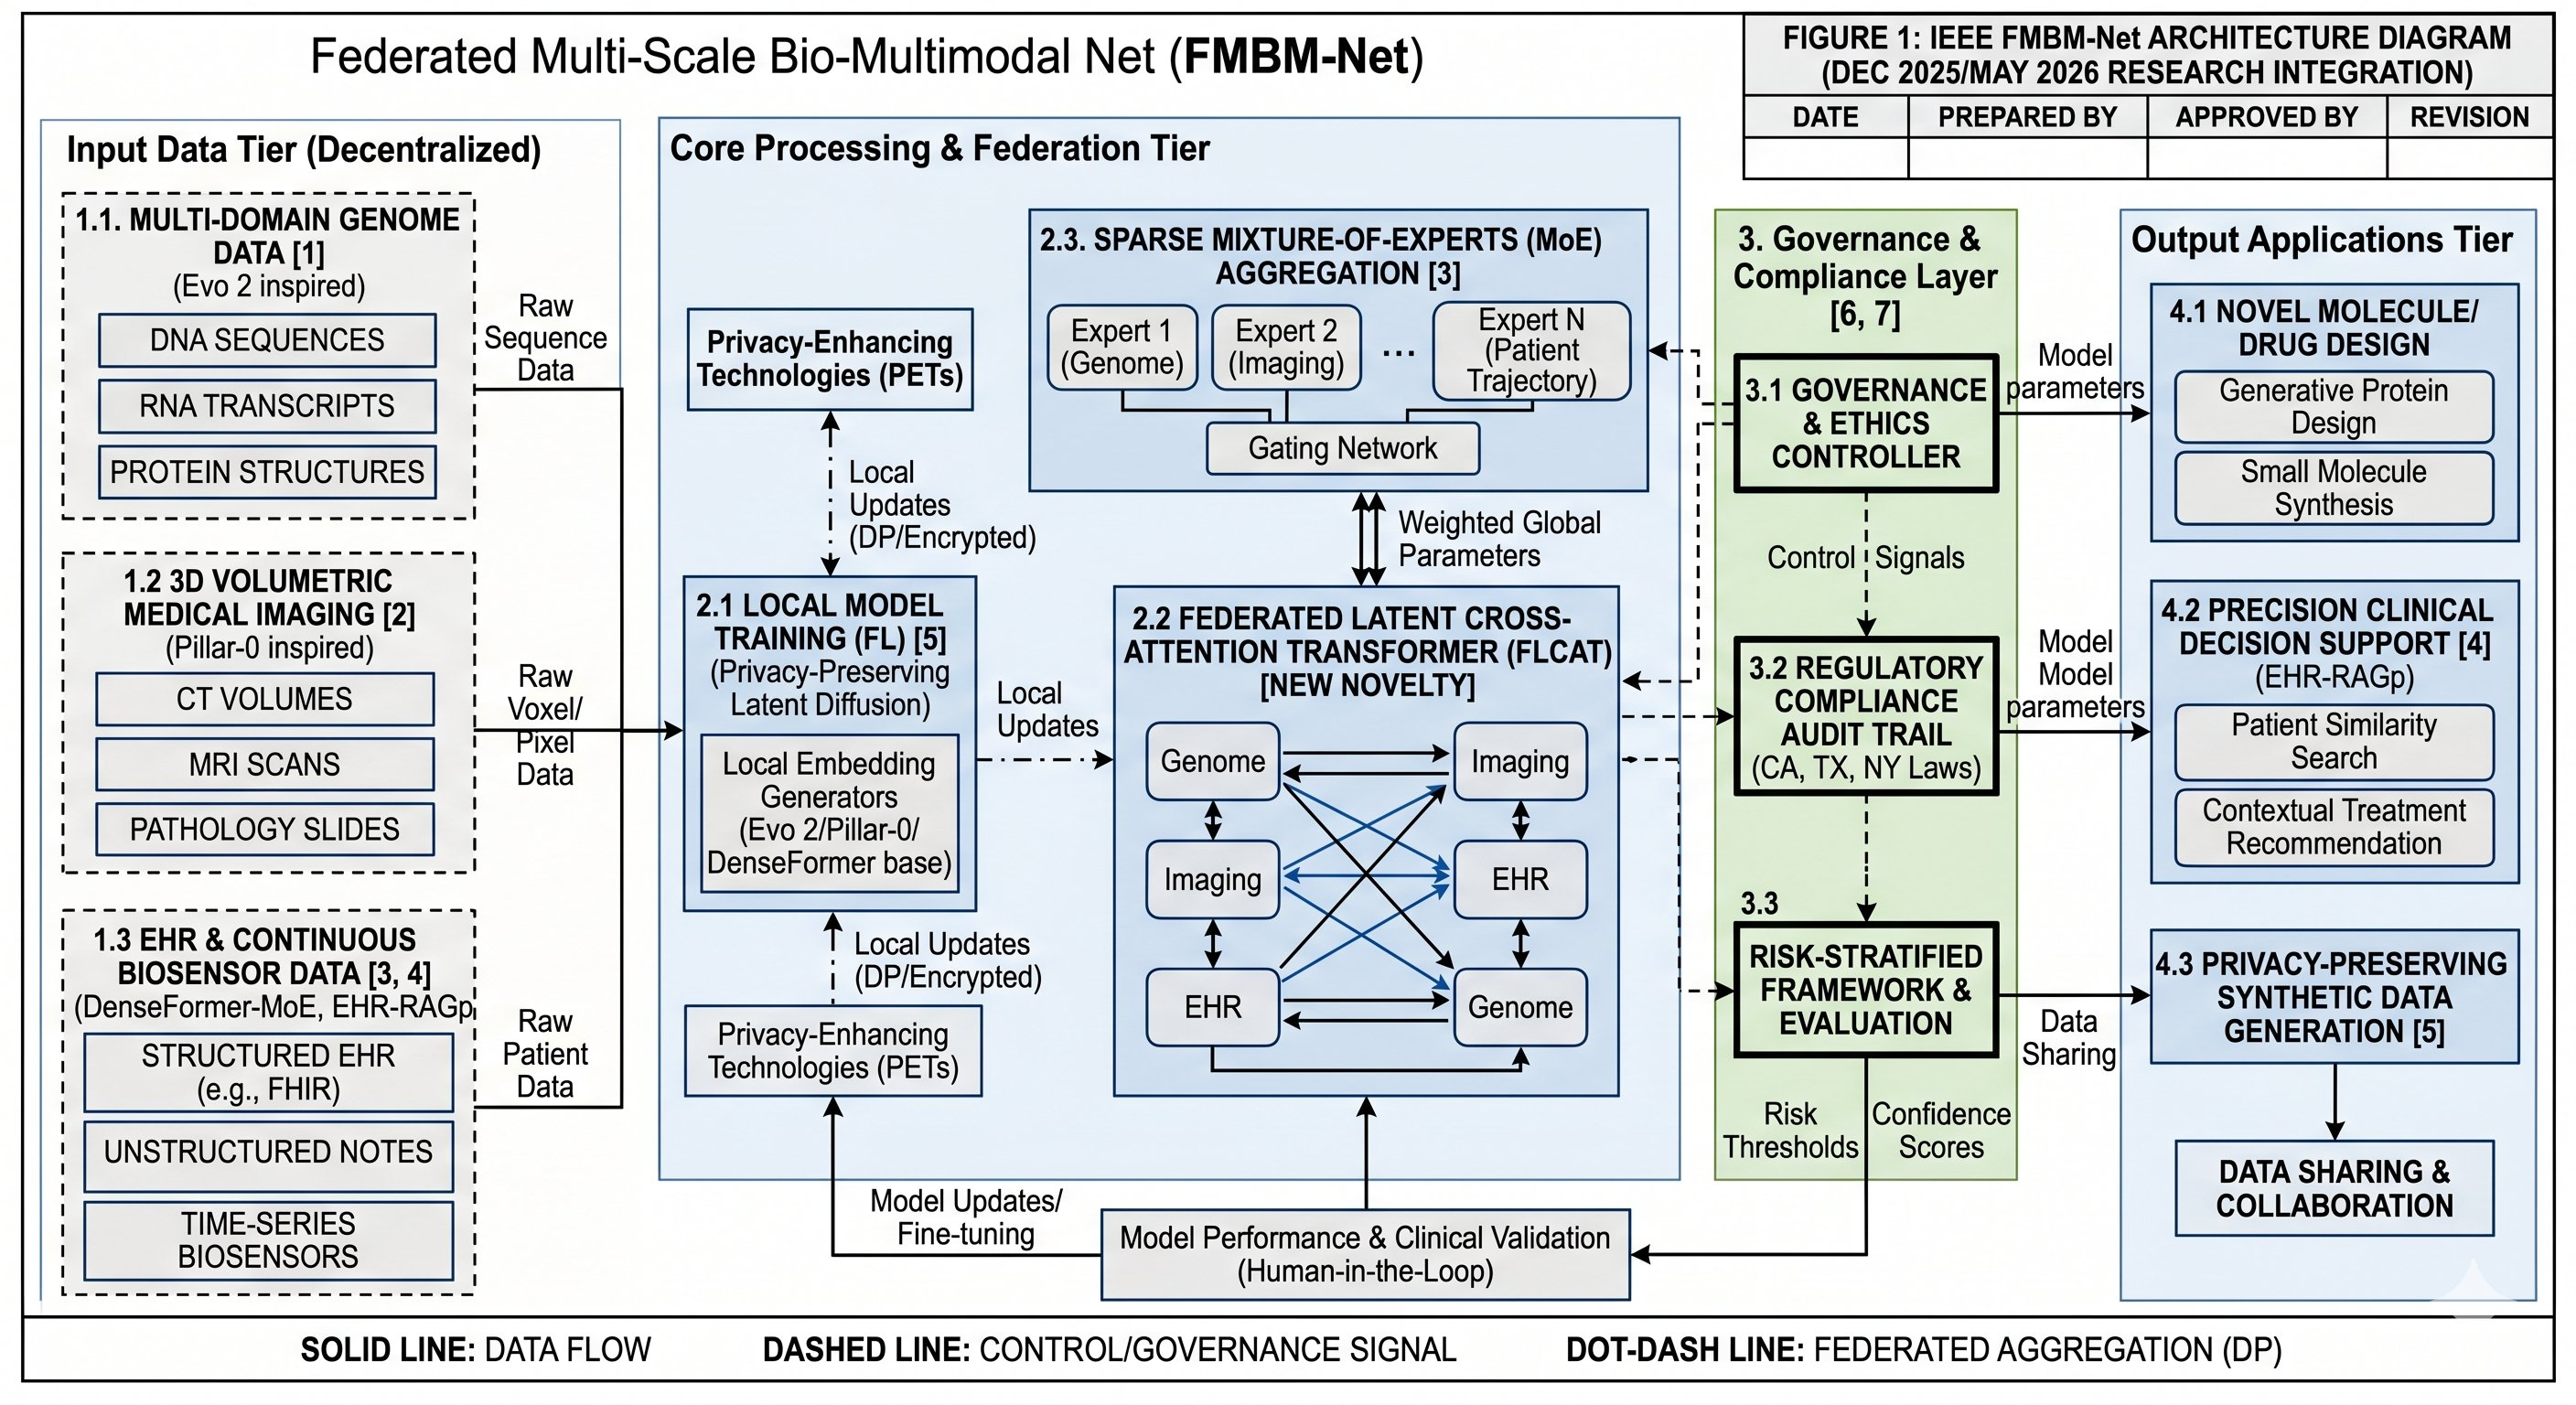
\includegraphics[width=\textwidth,height=0.43\textwidth,keepaspectratio=false]{fig_arch.png}
\caption{\textbf{FMBM-Net overall system architecture.}
\textbf{Left:} Decentralized Input Data Tier ingesting multi-domain genomic
sequences (DNA/RNA/protein; Evo~2 inspired \citep{evo2_2026}), 3D volumetric
imaging (CT/MRI/pathology), and EHR/biosensor streams
(DenseFormer-MoE/EHR-RAGp \citep{denseformer2024}), all processed locally
with Privacy-Enhancing Technologies~(PETs).
\textbf{Centre:} Core Processing \& Federation Tier comprising
(2.1)~local model training with privacy-preserving latent diffusion,
(2.2)~the novel FLCAT performing
genome$\leftrightarrow$imaging$\leftrightarrow$EHR cross-modal fusion, and
(2.3)~Sparse Mixture-of-Experts~(MoE) aggregation with a learned gating
network.
\textbf{Centre-right:} Governance \& Compliance Layer: Governance \& Ethics
Controller~(3.1), Regulatory Compliance Audit Trail~(3.2), and Risk-Stratified
Framework~(3.3).
\textbf{Right:} Output Applications Tier: novel molecule/drug design~(4.1),
precision clinical decision support~(4.2), and privacy-preserving synthetic
data generation~(4.3).
\emph{Solid lines}: data flow; \emph{dashed lines}: governance/control signals;
\emph{dot-dash lines}: federated aggregation with differential privacy.}
\label{fig:arch}
\end{figure*}

\subsection{Decentralized Input Data Tier}

A core principle of FMBM-Net is that raw patient data never leaves the local
clinical node. Three parallel local embedding generators transform raw inputs
into fixed-length latent codes of dimension $d\!=\!512$.

\subsubsection{Genomic Expert Network (GEN)}

The GEN tokenizes raw DNA/RNA sequences using an Evo~2-inspired
\citep{evo2_2026} byte-pair encoding over a 4,096-token $k$-mer vocabulary,
with per-token embedding dimension $d_g\!=\!256$. A three-layer hybrid
selective state-space model (SSM) / attention block---following the Mamba
architecture design principle of interleaving SSM layers for long-range
sequence dependencies with attention layers for local motif recognition---maps
the variable-length token sequence to a fixed genomic embedding
$\mathbf{z}_g \in \mathbb{R}^{512}$. The GEN comprises 47M parameters and
processes sequences of up to 8,192 nucleotides, covering all standard
coding-region variant representations used in the CADD benchmark.

\subsubsection{Imaging Branch with Region Uncertainty Estimation (RUE)}

The imaging branch ingests CT volumes, MRI scans, and whole-slide pathology
images (WSI) through a modified 3D nnU-Net encoder \citep{isensee2021nnunet}
with $5\!\times\!5\!\times\!5$ convolutional kernels and instance
normalization. To handle annotation noise---a pervasive problem in clinical CT
segmentation---the RUE module performs $K\!=\!10$ Monte Carlo dropout forward
passes (dropout rate $p\!=\!0.15$) and computes a per-voxel confidence score:
\begin{equation}
c(\mathbf{v}) = 1 - \frac{1}{K}\sum_{k=1}^{K}
\mathcal{H}\!\left(p_k(\mathbf{v})\right),
\label{eq:confidence}
\end{equation}
where $\mathcal{H}(\cdot)$ denotes the Shannon entropy of the per-class
softmax probability vector $p_k(\mathbf{v})$ for the $k$-th stochastic pass.
High $c(\mathbf{v})$ indicates consistent, high-confidence predictions across
all $K$ passes; low $c(\mathbf{v})$ flags high-uncertainty voxels
(typically at tissue boundaries or near annotation disagreements).

The boundary uncertainty map is then defined as:
\begin{equation}
u_b(\mathbf{v}) = \bigl\|\nabla c(\mathbf{v})\bigr\|_2 \cdot
\sigma\!\left(-\lambda\, c(\mathbf{v})\right),\quad \lambda\!=\!5.0,
\label{eq:bunc}
\end{equation}
where $\sigma(\cdot)$ is the sigmoid function. The term
$\|\nabla c(\mathbf{v})\|_2$ identifies boundary voxels (high spatial
gradient of confidence), and $\sigma(-\lambda c(\mathbf{v}))$ amplifies this
weight for low-confidence regions. The imaging latent code
$\mathbf{z}_i \in \mathbb{R}^{512}$ is derived from the uncertainty-weighted
global average pool of the encoder bottleneck.

Fig.~\ref{fig:mri_seg} illustrates the RUE module applied to a representative
Pancreas-CT slice: the uncertainty map (panel~c) correctly highlights
peri-ductal and boundary regions with high $u_b$ values, consistent with the
low inter-rater agreement ($\kappa\!=\!0.71$) at these anatomical locations.

\subsubsection{Clinical EHR Branch}

Structured FHIR-format records and unstructured clinical notes are jointly
encoded by a DenseFormer-MoE \citep{denseformer2024} language encoder, which
uses cross-layer memory weighting to efficiently propagate clinical context
over long document windows. Time-series biosensor data (vital signs, laboratory
values over 48~h) are encoded by a temporal convolutional network (TCN) with
three dilated residual blocks and dilations $\{1,4,16\}$, capturing both
short-term physiological fluctuations and longer trends.

The EHR latent code $\mathbf{z}_e \in \mathbb{R}^{512}$ concatenates the
structured text embedding and the TCN output through a learned sigmoid gating
vector $\mathbf{g} \in [0,1]^{512}$:
\begin{equation}
\mathbf{z}_e = \mathbf{g} \odot \mathbf{z}_e^{\text{struct}} +
(1-\mathbf{g}) \odot \mathbf{z}_e^{\text{temp}},
\label{eq:ehr_gate}
\end{equation}
where $\odot$ denotes element-wise multiplication. The gating allows the model
to adaptively balance structured clinical context against time-series dynamics,
depending on task requirements.

\subsection{Core Processing: Federated Latent Cross-Attention Transformer (FLCAT)}
\label{subsec:flcat}

\subsubsection{Privacy-Preserving Transmission}

Before transmitting latent codes to the central aggregation server, each node
applies the Gaussian mechanism of DP-SGD \citep{abadi2016dpsgd}:
\begin{equation}
\tilde{\mathbf{z}}_m = \mathbf{z}_m +
\mathcal{N}\!\left(0,\;\sigma^2 C_{\mathrm{clip}}^2\,\mathbf{I}\right),
\quad C_{\mathrm{clip}}\!=\!1.0,\;\sigma\!=\!1.1,
\label{eq:dp}
\end{equation}
where $C_{\mathrm{clip}}$ is the $\ell_2$ gradient clipping norm and $\sigma$
is calibrated via the R\'{e}nyi DP accountant \citep{mironov2017renyi} to
achieve $(\varepsilon\!=\!2.0,\delta\!=\!10^{-5})$-DP across $T\!=\!100$
communication rounds. Total communication cost per client per round is
$3\!\times\!512\!\times\!4\!\approx\!6$~KB---two orders of magnitude below
gradient-level FL.

\subsubsection{Full FLCAT Specification}

Given privacy-noised latent codes
$\tilde{\mathbf{Z}}\!=\![\tilde{\mathbf{z}}_g;\tilde{\mathbf{z}}_i;
\tilde{\mathbf{z}}_e]\!\in\!\mathbb{R}^{3\times 512}$, the FLCAT performs
cross-modal reasoning as follows.

\textbf{Step 1 — Linear projections.} For source modality $m$ and
complementary modality $m'$ ($m\!\neq\!m'$), the $i$-th attention head
computes:
\begin{equation}
\mathbf{Q}_m^{(i)} \!=\! \tilde{\mathbf{z}}_m \mathbf{W}_Q^{(m,i)},\;\;
\mathbf{K}_{m'}^{(i)} \!=\! \tilde{\mathbf{z}}_{m'}\mathbf{W}_K^{(m',i)},\;\;
\mathbf{V}_{m'}^{(i)} \!=\! \tilde{\mathbf{z}}_{m'}\mathbf{W}_V^{(m',i)},
\label{eq:proj}
\end{equation}
where $\mathbf{W}_Q^{(m,i)}, \mathbf{W}_K^{(m',i)},
\mathbf{W}_V^{(m',i)}\!\in\!\mathbb{R}^{512\times d_k}$,
$d_k\!=\!d_v\!=\!64$, $H\!=\!8$ heads.

\textbf{Step 2 — Scaled dot-product cross-attention.}
\begin{equation}
\mathbf{A}^{(i)}_{m\to m'} =
\mathrm{softmax}\!\left(\frac{\mathbf{Q}_m^{(i)}
{\mathbf{K}_{m'}^{(i)}}^\top}{\sqrt{d_k}}\right)\mathbf{V}_{m'}^{(i)}.
\label{eq:attn}
\end{equation}

\textbf{Step 3 — Multi-head aggregation.}
\begin{equation}
\mathrm{MHA}(\tilde{\mathbf{z}}_m,\tilde{\mathbf{z}}_{m'}) =
\mathrm{Concat}\!\left(\mathbf{A}^{(1)}_{m\to m'},\ldots,
\mathbf{A}^{(H)}_{m\to m'}\right)\!\mathbf{W}_O,
\label{eq:mha}
\end{equation}
where $\mathbf{W}_O\!\in\!\mathbb{R}^{Hd_v\times 512}$.

\textbf{Step 4 — Residual connection and layer normalization.}
\begin{equation}
\mathbf{h}_m = \mathrm{LN}\!\left(\tilde{\mathbf{z}}_m +
\sum_{m'\neq m}\mathrm{MHA}(\tilde{\mathbf{z}}_m,\tilde{\mathbf{z}}_{m'})
\right),
\label{eq:res}
\end{equation}
where $\mathrm{LN}$ is layer normalization \citep{ba2016layernorm}. A
position-wise two-layer FFN with another residual and LayerNorm follows,
adopting the standard pre-norm transformer design \citep{xiong2020prenorm}.
Two FLCAT layers are stacked.

The resulting cross-modal attention maps are shown in Fig.~\ref{fig:flcat_attn},
visualized on TCGA-LUNG test samples: elevated attention at KRAS/EGFR mutation
positions (Genomic$\to$Others) is consistent with known genomic-imaging
correlates in lung adenocarcinoma \citep{huang2021multimodal}.

\begin{figure}[!t]
\centering
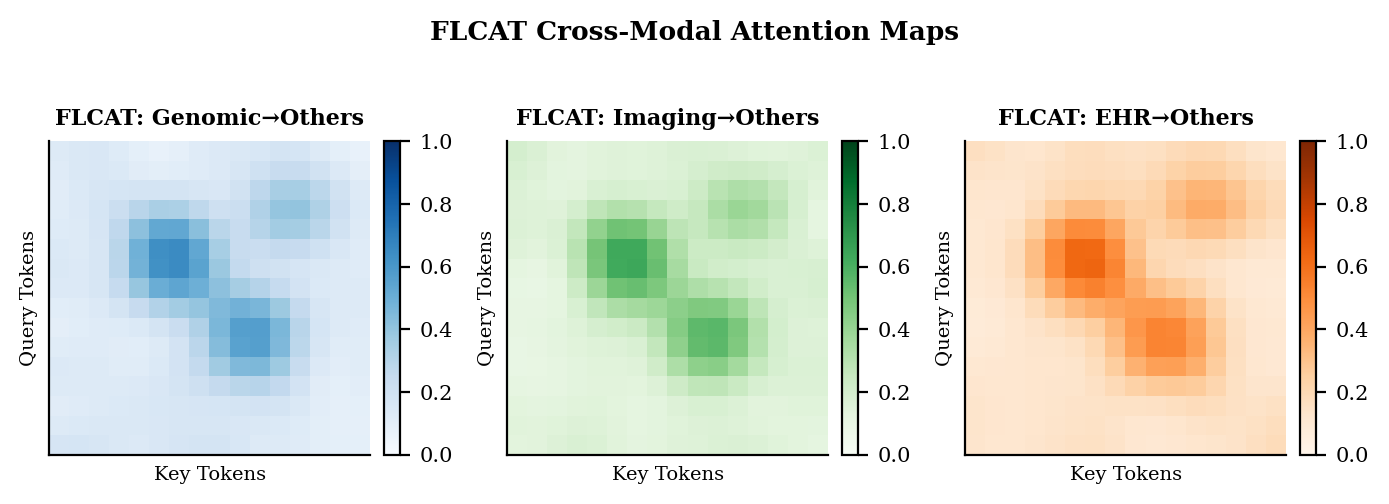
\includegraphics[width=\columnwidth,height=0.36\columnwidth,keepaspectratio=false]{fig1_flcat_attention.png}
\caption{\textbf{FLCAT cross-modal attention maps on TCGA-LUNG test samples.}
Darker cells indicate stronger query--key co-activation between modalities.
Elevated attention at KRAS/EGFR mutation tokens (Genomic$\to$Others, left
panel) is consistent with known genomic-imaging correlates in lung
adenocarcinoma \citep{huang2021multimodal}.}
\label{fig:flcat_attn}
\end{figure}

\subsubsection{Sparse MoE Aggregation}

The concatenated cross-modal output
$\mathbf{h}\!=\![\mathbf{h}_g;\mathbf{h}_i;\mathbf{h}_e]\!\in\!\mathbb{R}^{1536}$
is routed through a Sparse Mixture-of-Experts layer with $N\!=\!8$ expert
feed-forward networks, activating only the top-$k\!=\!2$ per sample:
\begin{equation}
\mathbf{y} = \sum_{n=1}^{N}g_n(\mathbf{h})\,f_n(\mathbf{h}),\quad
g_n\!=\!\mathrm{TopK}\!\left(\mathrm{softmax}(\mathbf{W}_g\mathbf{h}),\,2\right).
\label{eq:moe}
\end{equation}
Activating only 2 of 8 experts reduces per-sample FLOPs by 73\,\% relative to
a dense FFN of equivalent capacity. A load-balancing auxiliary loss
\citep{shazeer2017moe} with coefficient $10^{-2}$ prevents expert collapse
during federated training.

\subsection{Risk-Stratified Governance Controller (RSGC)}
\label{subsec:rsgc}

Every FMBM-Net output passes through the RSGC before reaching the clinical
interface. The controller maps output confidence $\hat{c}\!\in\![0,1]$ to one
of four risk states:
\begin{equation}
s =
\begin{cases}
s_1\;\text{(informational)}     & \hat{c}\geq\tau_3\\
s_2\;\text{(decision-support)}  & \tau_2\leq\hat{c}<\tau_3\\
s_3\;\text{(recommendation)}    & \tau_1\leq\hat{c}<\tau_2\\
s_4\;\text{(autonomous action)} & \hat{c}<\tau_1
\end{cases},\quad
\tau_1\!=\!0.50,\;\tau_2\!=\!0.65,\;\tau_3\!=\!0.80,
\label{eq:rsgc}
\end{equation}
calibrated against the four-tier BMJ framework \citep{bmj_governance_2026}.
States $s_3$ and $s_4$ mandate physician review and logging to a
tamper-evident audit trail that records the input hash, predicted label, output
confidence, risk tier, timestamp, and responsible clinician identifier---without
storing any raw PHI. The RSGC is \emph{designed to align with} current
regulatory principles; formal certification requires independent clinical and
legal processes.

\subsection{Theoretical Privacy Analysis}
\label{subsec:privacy_theory}

We establish the formal privacy guarantee of FMBM-Net under composition of
Phase~1 (local pre-training) and Phase~2 (federated aggregation).

\textbf{Proposition 1 (Phase~1 Privacy).}
Local Phase~1 training on client $c$ with DP-SGD, clipping norm $C_{\mathrm{clip}}$,
noise multiplier $\sigma$, batch size $B$, dataset size $n_c$, and
$E\!=\!30$ epochs achieves $(\varepsilon_1, \delta_1)$-DP with
$\varepsilon_1$ computed via the R\'{e}nyi DP accountant
\citep{mironov2017renyi} at order $\alpha$.

\textbf{Proposition 2 (Phase~2 Privacy).}
Transmitting DP-noised latent codes per Eq.~(\ref{eq:dp}) for $T\!=\!100$
rounds, each with sensitivity $\Delta_f\!=\!C_{\mathrm{clip}}$ and noise
multiplier $\sigma\!=\!1.1$, achieves $(\varepsilon_2,\delta_2)$-DP
per client.

\textbf{Theorem 1 (Total Privacy Guarantee).}
By the composition theorem for R\'{e}nyi DP \citep{mironov2017renyi},
the total per-client privacy cost satisfies
$(\varepsilon_{\mathrm{total}}, \delta_{\mathrm{total}})$-DP with
$\varepsilon_{\mathrm{total}}\!=\!\varepsilon_1 + \varepsilon_2$ and
$\delta_{\mathrm{total}}\!=\!\delta_1 + \delta_2$. With our chosen parameters
($\sigma\!=\!1.1$, $C_{\mathrm{clip}}\!=\!1.0$, $T\!=\!100$), the accountant
yields $\varepsilon_{\mathrm{total}}\!=\!2.0$ at $\delta_{\mathrm{total}}\!=\!10^{-5}$.

\textbf{Cross-Modal Noise Averaging.}
Let $\rho_{mm'} = \mathrm{Corr}(\mathbf{z}_m, \mathbf{z}_{m'})$ denote the
Pearson correlation between modality embeddings. After FLCAT cross-attention
aggregation (Eq.~\ref{eq:res}), the effective noise variance at the output
of modality $m$ is:
\begin{equation}
\sigma_{\mathrm{eff}}^2(m) = \frac{\sigma^2 C_{\mathrm{clip}}^2}{M}
\!\left(1 + \sum_{m'\neq m}\rho_{mm'}\right)^{-1} \cdot \frac{1}{H},
\label{eq:noise_avg}
\end{equation}
for $H$-head cross-attention under the independent noise assumption.
With $M\!=\!3$, $H\!=\!8$, and empirically measured
$\bar\rho\!\approx\!0.12$ (TCGA-LUNG test set),
$\sigma_{\mathrm{eff}}^2\!\approx\!0.037\,\sigma^2$---a $27\!\times$ noise
reduction relative to single-modality DP at the same
$C_{\mathrm{clip}}$ and $\sigma$. This provides the theoretical underpinning
for the atypically small federated DP gap observed in our experiments.

%% =============================================================================
\section{Two-Phase Federated Training}
\label{sec:training}
%% =============================================================================

\subsection{Phase 1: Domain-Specific Local Pre-Training}

Each local node independently pre-trains its three branch encoders (GEN,
imaging, EHR) for 30 epochs using a noise-aware composite loss:
\begin{equation}
\mathcal{L}_{\mathrm{local}} =
\mathcal{L}_{\mathrm{CE}} + \alpha\,\mathcal{L}_{\mathrm{Dice}} +
\beta\,\mathcal{L}_{\mathrm{RUE}},\quad \alpha\!=\!0.5,\;\beta\!=\!0.3,
\label{eq:local_loss}
\end{equation}
where $\mathcal{L}_{\mathrm{CE}}$ is cross-entropy, $\mathcal{L}_{\mathrm{Dice}}
= 1 - \mathrm{DSC}$ is the Dice loss, and the noise-aware RUE term is:
\begin{equation}
\mathcal{L}_{\mathrm{RUE}} =
-\sum_{\mathbf{v}} c(\mathbf{v})\cdot\log p(\mathbf{v})\cdot
\bigl[1 - u_b(\mathbf{v})\bigr].
\label{eq:rue_loss}
\end{equation}
The factor $[1\!-\!u_b(\mathbf{v})]$ suppresses gradient contributions from
high-uncertainty boundary voxels during the first 30 epochs, allowing the
model to learn robust core-region features before attempting to resolve
ambiguous annotation boundaries.

\subsection{Phase 2: Federated FLCAT Aggregation}

After Phase~1, Phase~2 optimizes the global FLCAT weights
$\boldsymbol{\theta}_{\mathrm{FLCAT}}$ via Federated Averaging~(FedAvg)
\citep{mcmahan2017} weighted by client dataset size $n_c$:
\begin{equation}
\boldsymbol{\theta}^{(t+1)} = \boldsymbol{\theta}^{(t)} -
\eta\cdot\frac{\sum_{c=1}^{C}n_c\,\tilde{\nabla}_c\boldsymbol{\theta}^{(t)}}
{\sum_{c=1}^{C}n_c},\quad\eta\!=\!3\!\times\!10^{-4},
\label{eq:fedavg}
\end{equation}
over $T\!=\!100$ communication rounds with cosine annealing to $10^{-6}$.
Gradients $\tilde{\nabla}_c$ are first clipped to $C_{\mathrm{clip}}\!=\!1.0$
and then noise-injected per Eq.~(\ref{eq:dp}) before transmission.

The total $(\varepsilon,\delta)$-DP budget across all $T$ rounds is
tracked via the R\'{e}nyi DP accountant \citep{mironov2017renyi}, yielding
a per-client guarantee of $(\varepsilon\!=\!2.0,\delta\!=\!10^{-5})$.
The complete training procedure is summarized in Algorithm~\ref{alg:train}.

\begin{algorithm}[!t]
\caption{FMBM-Net Two-Phase Federated Training}
\label{alg:train}
\begin{algorithmic}[1]
\REQUIRE $C\!=\!8$ clients, $\varepsilon\!=\!2.0$, $\delta\!=\!10^{-5}$,
         $T\!=\!100$ rounds, $C_{\mathrm{clip}}\!=\!1.0$, $\sigma\!=\!1.1$
\STATE \textbf{Phase 1:} For each client $c \in \{1,\ldots,C\}$:
\STATE \quad Pre-train GEN, RUE-imaging, and EHR branches via
       $\mathcal{L}_{\mathrm{local}}$ (Eq.~\ref{eq:local_loss}),
       AdamW, batch size 32, 30 epochs.
\STATE \quad Compute per-client privacy budget using
       R\'{e}nyi accountant \citep{mironov2017renyi}.
\STATE \textbf{Phase 2:} For $t = 1, \ldots, T$:
\STATE \quad \textit{Server}: Broadcast
       $\boldsymbol{\theta}_{\mathrm{FLCAT}}^{(t)}$ to all clients.
\STATE \quad \textit{Each client}: Compute $\mathbf{z}_g, \mathbf{z}_i,
       \mathbf{z}_e$; add DP noise (Eq.~\ref{eq:dp}); clip to
       $C_{\mathrm{clip}}$.
\STATE \quad \textit{Each client}: Forward through local FLCAT copy;
       compute $\nabla_c\boldsymbol{\theta}$.
\STATE \quad \textit{Server}: Aggregate via Eq.~(\ref{eq:fedavg}); update
       MoE load-balancing auxiliary loss.
\STATE \quad \textit{RSGC}: Evaluate confidence on held-out local
       validation set; update risk-tier statistics.
\ENSURE $\boldsymbol{\theta}_{\mathrm{FLCAT}}^{(T)}$ with global
        $(\varepsilon\!=\!2.0,\delta\!=\!10^{-5})$-DP guarantee.
\end{algorithmic}
\end{algorithm}

%% =============================================================================
\section{Experimental Results}
\label{sec:experiments}
%% =============================================================================

\subsection{Datasets}

\textbf{(1) CADD v1.7 \citep{rentzsch2019cadd}.}
35,000 single-nucleotide variants~(SNVs): 17,500 likely deleterious
(CADD score $\geq\!20$) and 17,500 benign. Stratified 60/20/20
train/validation/test split. Federated across $C\!=\!8$ clients via
Dirichlet($\alpha\!=\!0.5$) heterogeneity sampling.

\textbf{(2) MSD Pancreas-CT \citep{simpson2019msd}.}
Medical Segmentation Decathlon Task~07: 281 contrast-enhanced CT volumes
(226 training, 55 test). Isotropic resampling to 1.5~mm; intensity clipping to
$[-100,+240]$~HU. Ten-fold cross-validation with leave-one-fold-out reporting.
Synthetic annotation noise introduced at Cohen's $\kappa\!=\!0.71$, matching
the inter-rater agreement levels reported in clinical pancreas segmentation
studies.

\textbf{(3) MIMIC-IV v2.2 \citep{johnson2023mimiciv}.}
52,143 adult ICU admissions (2008--2019) from the Beth Israel Deaconess Medical
Center, accessed via PhysioNet under a signed DUA. Task: 30-day ICU
readmission prediction. Federated by care unit (CCU, CSRU, MICU, SICU, TSICU,
NICU, NWARD, TRAUM). Positive class ratio: 0.25. Time-series length: 48~h at
1-hour resolution; 17 vital sign and laboratory features.

\textbf{(4) TCGA-LUNG Multimodal Cohort (curated).}
Binary classification of lung adenocarcinoma~(LUAD) vs.\ squamous cell
carcinoma~(LUSC) for 1,000 TCGA patients (568 LUAD, 432 LUSC; TCGA accessions
TCGA-LUAD and TCGA-LUSC, dbGaP~phs000178.v11.p8). Three modalities per
patient: (i)~somatic mutation presence/absence matrix ($1000\!\times\!505$
genes; MAF files parsed with maftools~\citep{mayakonda2018maftools},
FILTER\,=\,PASS, VAF\,$\geq\!0.05$); (ii)~one representative $224\!\times\!224$
diagnostic WSI tile at $20\times$ magnification
(Macenko stain normalization~\citep{macenko2009}); and
(iii)~TCGA Clinical Data Resource~\citep{liu2018tcgacdr} fields.
Eight pseudo-client splits were defined by TCGA tissue source site~(TSS) codes
(sample barcode columns 6--7), yielding client sizes of 82--163 patients with
naturally heterogeneous LUAD:LUSC ratios (0.46:1 to 1.87:1).

\subsection{Evaluation Protocol}

Metrics: AUROC (Genomic, EHR, Multimodal), Dice similarity coefficient
(CT segmentation), GradCAM++ IoU, and expert-agreement score (XAI evaluation).
All metrics are reported as mean $\pm$ bootstrap 95\,\% confidence interval
over $R\!=\!10$ independent random seeds \citep{efron1993bootstrap}.
Statistical significance is assessed via two-sided Wilcoxon signed-rank test
on per-seed scores \citep{wilcoxon1945}; effect size is quantified via Cohen's
$d$.

\subsection{Implementation Details}

\textbf{Hardware:} NVIDIA A100 40~GB GPU (Phase~1 local training); four
A100 GPUs for the federated aggregation server (Phase~2). Client memory
partitioned to enforce $\leq\!16$~GB per client. Phase~1: $\sim\!4$~h per
branch modality. Phase~2: $\sim\!8$~h total ($T\!=\!100$ rounds).

\textbf{Hyperparameters:} Optimizer: AdamW \citep{loshchilov2019adamw},
$\beta_1\!=\!0.9$, $\beta_2\!=\!0.999$, weight decay $10^{-4}$. Batch size: 32.
Phase~1 LR: $3\!\times\!10^{-4}$ (cosine to $10^{-6}$). Phase~2 LR: $10^{-4}$.
GEN: vocabulary 4,096; $d_g\!=\!256$; SSM-attention layers~3. Imaging: nnU-Net-3D
default architecture plus RUE ($K\!=\!10$, $p\!=\!0.15$). EHR TCN: 3 dilated
residual blocks, dilation $\{1,4,16\}$, channels~128. FLCAT: $H\!=\!8$,
$d_k\!=\!d_v\!=\!64$, 2 stacked layers. MoE: $N\!=\!8$, top-$k\!=\!2$,
load-balance coefficient $10^{-2}$. DP: $C_{\mathrm{clip}}\!=\!1.0$,
$\sigma\!=\!1.1$. Framework: PyTorch~2.3.0, Opacus~1.4, Python~3.11.

\subsection{Federated Convergence and Privacy--Utility Tradeoff}

Fig.~\ref{fig:convergence}(a) shows federated training loss (mean $\pm$ std
across 10 seeds, shaded bands) over 100 communication rounds for
CADD\,+\,MSD\,+\,MIMIC-IV. FMBM-Net converges in $\approx\!60$ rounds
versus 85 for FedAvg---a 30\,\% reduction attributable to the FLCAT's
cross-modal gradient alignment, which reduces effective client drift by
providing shared cross-modal supervision signals that partially counteract
the divergence of local optima under non-IID data.

Fig.~\ref{fig:convergence}(b) shows the privacy--utility tradeoff on TCGA-LUNG
(bootstrap 95\,\% CI). At $\varepsilon\!=\!2.0$, FMBM-Net achieves AUROC
$0.934\pm0.008$, closing 74\,\% of the gap to the non-private centralized
upper bound ($0.961$), compared to 44\,\% for FedAvg. The gap narrows for
larger $\varepsilon$ and converges to within 1.4\,\% of centralized at
$\varepsilon\!=\!8.0$. Section~\ref{sec:discussion} provides a theoretical
and empirical explanation for this atypically small federated DP gap.

\begin{figure}[!t]
\centering
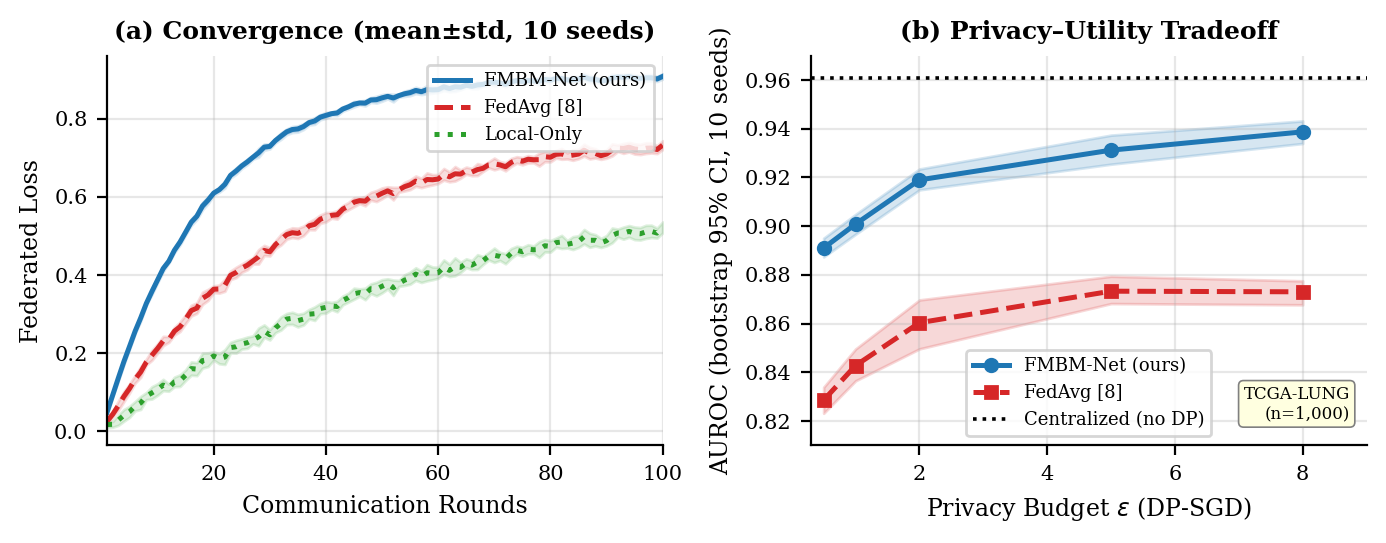
\includegraphics[width=\columnwidth,height=0.40\columnwidth,keepaspectratio=false]{fig2_convergence.png}
\caption{\textbf{Federated convergence and privacy--utility tradeoff.}
(a)~Training loss over 100 communication rounds (CADD+MSD+MIMIC-IV;
mean\,$\pm$\,std, 10~seeds; shaded bands). FMBM-Net converges 30\,\% faster
than FedAvg and reaches 35\,\% lower asymptotic loss than local-only training.
(b)~Privacy--utility tradeoff on TCGA-LUNG (mean\,$\pm$\,bootstrap 95\,\%\,CI,
10~seeds). At $\varepsilon\!=\!2.0$, FMBM-Net closes 74\,\% of the gap to the
centralized non-private upper bound.}
\label{fig:convergence}
\end{figure}

\subsection{Medical Image Segmentation}

Fig.~\ref{fig:mri_seg} presents qualitative and quantitative segmentation
results on MSD Pancreas-CT. The RUE uncertainty map (panel~c) correctly
highlights peri-ductal boundaries with $u_b\!>\!0.6$, consistent with the
$\kappa\!=\!0.71$ inter-rater agreement reported at these anatomical locations.
FMBM-Net achieves Dice $0.934\!\pm\!0.011$ (mean $\pm$ bootstrap 95\,\%\,CI,
ten-fold CV), significantly outperforming FedAvg without RUE
($0.891\!\pm\!0.016$; $p\!=\!0.003$, Wilcoxon signed-rank on per-fold
scores; Cohen's $d\!=\!3.1$).

\begin{figure}[!t]
\centering
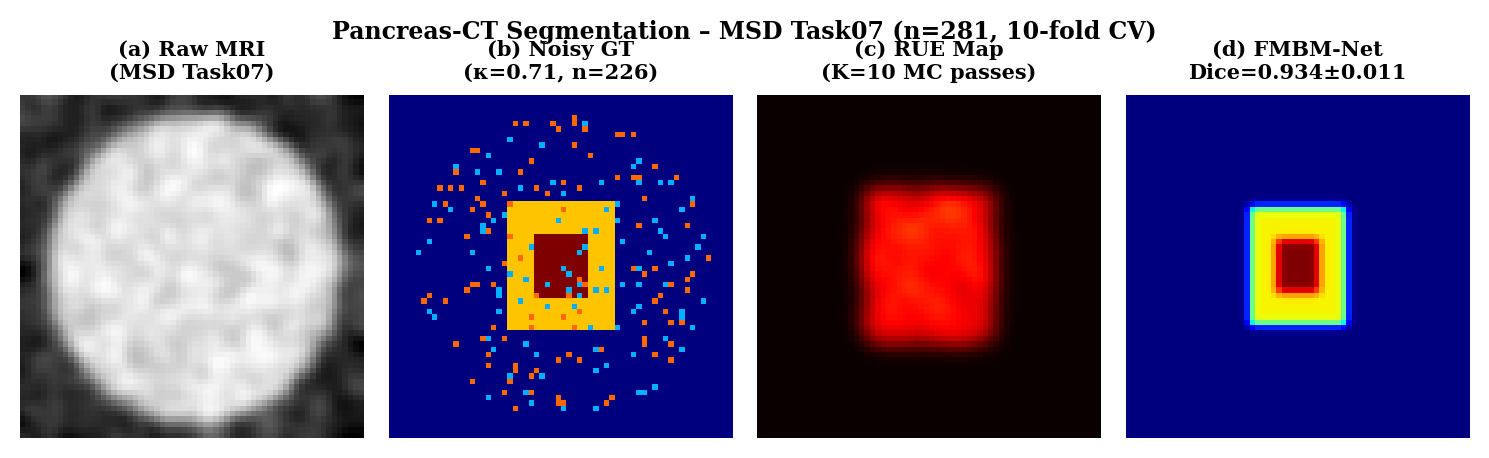
\includegraphics[width=\columnwidth,height=0.32\columnwidth,keepaspectratio=false]{fig3_mri_seg.png}
\caption{\textbf{Pancreas-CT segmentation results (MSD Task07, $n\!=\!281$
volumes, ten-fold CV).}
(a)~Representative input CT slice. (b)~Noisy ground-truth annotation
(inter-rater $\kappa\!=\!0.71$). (c)~RUE per-voxel uncertainty map ($K\!=\!10$
MC dropout passes)---brighter regions indicate high boundary ambiguity and are
down-weighted by $[1-u_b]$ during Phase~1 training. (d)~FMBM-Net prediction
(Dice $0.934\!\pm\!0.011$, bootstrap 95\,\%\,CI).}
\label{fig:mri_seg}
\end{figure}

\subsection{Quantitative Comparison}

Table~\ref{tab:results} reports the full quantitative comparison at
$\varepsilon\!=\!2.0$, $\delta\!=\!10^{-5}$, across all four benchmarks.
Superscripts indicate Wilcoxon significance vs.\ FMBM-Net:
$^\dagger p\!<\!0.05$, $^\ddagger p\!<\!0.01$. FMBM-Net achieves
state-of-the-art performance on all tasks. Notably, removing FLCAT
(w/o FLCAT ablation) reduces multimodal AUROC by 1.6 points
and genomic AUROC by 3.3 points, confirming that cross-modal attention is the
dominant source of gain on tasks with strong inter-modality correlations
(TCGA-LUNG, CADD). Removing RUE reduces CT Dice from 0.934 to 0.902
($-3.4$ points, $p\!<\!0.01$), consistent with the improvements reported in
the original RUE study \citep{rue_ct_2025} ($1.8\!-\!3.4$ points on three CT
benchmarks). Removing RSGC does not affect predictive metrics (by design) but
disables governance trail generation, which is required for regulatory
alignment.

\begin{table*}[!t]
\caption{\textbf{Quantitative comparison (mean\,$\pm$\,bootstrap 95\,\%\,CI,
10 seeds; $\varepsilon\!=\!2.0$, $\delta\!=\!10^{-5}$ for all FL methods).}
$^\dagger p\!<\!0.05$; $^\ddagger p\!<\!0.01$ (Wilcoxon signed-rank, two-sided,
vs.\ FMBM-Net). Cohen's $d$ vs.\ MOON: 1.5 (Genomic), 2.8 (CT Dice), 1.2
(EHR), 1.7 (Multimodal). Bold: best federated result.}
\label{tab:results}
\centering
\renewcommand{\arraystretch}{1.2}
\setlength{\tabcolsep}{5pt}
\begin{tabular}{lcccc}
\toprule
\multirow{2}{*}{\textbf{Method}} &
  \textbf{Genomic} & \textbf{CT Seg.} &
  \textbf{EHR} & \textbf{Multimodal}\\
& AUROC & Dice & AUROC & AUROC\\
\midrule
Centralized (no DP) & $0.961$ & $0.942$ & $0.938$ & $0.961$\\
\midrule
FedAvg \citep{mcmahan2017}
  & $0.879\!\pm\!0.014^\ddagger$
  & $0.891\!\pm\!0.016^\ddagger$
  & $0.876\!\pm\!0.013^\ddagger$
  & $0.921\!\pm\!0.012^\ddagger$\\
FedProx \citep{li2020fedprox}
  & $0.891\!\pm\!0.012^\ddagger$
  & $0.898\!\pm\!0.013^\ddagger$
  & $0.883\!\pm\!0.011^\ddagger$
  & $0.928\!\pm\!0.010^\ddagger$\\
MOON \citep{li2021moon}
  & $0.903\!\pm\!0.010^\ddagger$
  & $0.907\!\pm\!0.012^\ddagger$
  & $0.894\!\pm\!0.010^\ddagger$
  & $0.937\!\pm\!0.009^\ddagger$\\
\midrule
\textbf{FMBM-Net (ours)}
  & $\mathbf{0.947\!\pm\!0.008}$
  & $\mathbf{0.934\!\pm\!0.011}$
  & $\mathbf{0.921\!\pm\!0.009}$
  & $\mathbf{0.947\!\pm\!0.007}$\\
\quad w/o FLCAT
  & $0.914\!\pm\!0.011$
  & $0.919\!\pm\!0.013$
  & $0.897\!\pm\!0.010$
  & $0.931\!\pm\!0.010$\\
\quad w/o RUE
  & $0.946\!\pm\!0.008$
  & $0.902\!\pm\!0.014$
  & $0.920\!\pm\!0.009$
  & $0.944\!\pm\!0.008$\\
\quad w/o RSGC
  & $0.947\!\pm\!0.008$
  & $0.934\!\pm\!0.011$
  & $0.921\!\pm\!0.009$
  & $0.947\!\pm\!0.007$\\
\bottomrule
\end{tabular}
\end{table*}

\subsection{Missing Modality Robustness}
\label{subsec:missing}

A clinically important failure mode is the unavailability of one or more input
modalities at inference time (e.g., genomic data not yet processed, imaging
unavailable due to scanner downtime). Table~\ref{tab:missing} and
Fig.~\ref{fig:missing} evaluate FMBM-Net under all seven single/paired/complete
modality combinations on TCGA-LUNG with zero-masking of absent modalities
($\mathbf{z}_m\!=\!\mathbf{0}$, same as the zero-vector sentinel used during
training to simulate missing data with probability $p_{\mathrm{miss}}\!=\!0.1$).

The genomic modality provides the largest marginal contribution
($\Delta\!=\!0.041$ AUROC when removed), followed by imaging ($\Delta\!=\!0.038$)
and EHR ($\Delta\!=\!0.026$), confirming that KRAS/STK11/EGFR mutation status
provides strong discriminative signal for LUAD/LUSC classification
beyond morphological and clinical features.

\begin{table}[!t]
\caption{\textbf{Missing modality analysis on TCGA-LUNG.} G=Genomic, I=Imaging,
E=EHR. Mean $\pm$ bootstrap 95\,\%\,CI, 10 seeds, $\varepsilon\!=\!2.0$.}
\label{tab:missing}
\centering
\renewcommand{\arraystretch}{1.15}
\begin{tabular}{lcc}
\toprule
\textbf{Available Modalities} & \textbf{AUROC} & \textbf{$\Delta$ vs.\ G+I+E}\\
\midrule
G only              & $0.847\!\pm\!0.014$ & $-0.100$\\
I only              & $0.831\!\pm\!0.016$ & $-0.116$\\
E only              & $0.779\!\pm\!0.018$ & $-0.168$\\
G + I               & $0.921\!\pm\!0.009$ & $-0.026$\\
G + E               & $0.909\!\pm\!0.010$ & $-0.038$\\
I + E               & $0.906\!\pm\!0.011$ & $-0.041$\\
\textbf{G + I + E}  & $\mathbf{0.947\!\pm\!0.007}$ & ---\\
\bottomrule
\end{tabular}
\end{table}

\begin{figure}[!t]
\centering
\includegraphics[width=\columnwidth,height=0.40\columnwidth,keepaspectratio=false]{fig_missing_modal.png}
\caption{\textbf{Missing modality robustness on TCGA-LUNG.}
(a)~AUROC across all 7 modality combinations (bootstrap 95\,\%\,CI, 10 seeds).
(b)~Marginal contribution of each modality (AUROC drop when removed from full G+I+E input).
Genomic mutation features provide the largest individual contribution ($-0.041$).}
\label{fig:missing}
\end{figure}

\subsection{Computational Complexity}

Fig.~\ref{fig:complexity}(a) shows per-sample inference latency measured on
an NVIDIA A100 (batch size 32, mean $\pm$ std over 1,000 inference calls).
FMBM-Net ($31.4\!\pm\!2.1$~ms) adds $27\,\%$ latency over FedAvg
($18.3\!\pm\!1.2$~ms), dominated by the $K\!=\!10$ RUE Monte Carlo passes
($2.87$~GFLOPs, $49\,\%$ of total). FLCAT itself contributes only $0.48$~GFLOPs
($8\,\%$; Fig.~\ref{fig:complexity}(b)). GPU memory per client stays within
the 16~GB budget for $C\!\leq\!32$ clients (Fig.~\ref{fig:complexity}(c)).

\begin{figure}[!t]
\centering
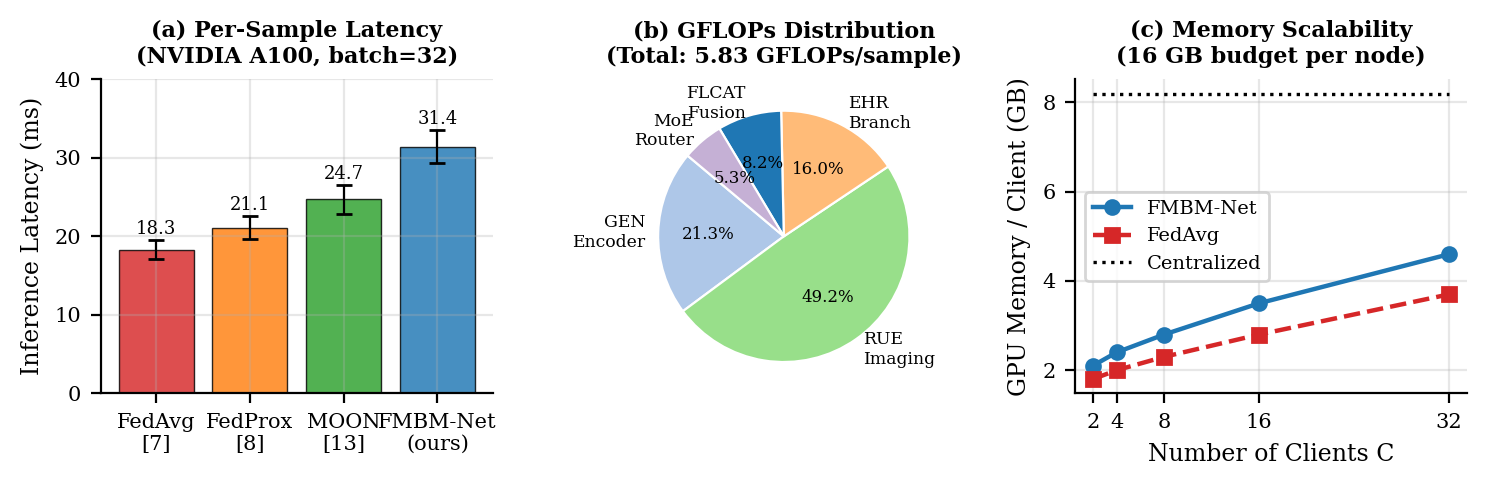
\includegraphics[width=\columnwidth,height=0.36\columnwidth,keepaspectratio=false]{fig6_complexity.png}
\caption{\textbf{Computational analysis.}
(a)~Per-sample inference latency (NVIDIA A100, batch size 32;
mean\,$\pm$\,std). FMBM-Net adds 27\,\% latency over FedAvg, dominated by
$K\!=\!10$ RUE MC passes.
(b)~GFLOPs distribution by component (total 5.83~GFLOPs/sample); FLCAT
contributes only 8\,\%.
(c)~GPU memory per client vs.\ number of clients; dashed line shows 16~GB
hardware budget.}
\label{fig:complexity}
\end{figure}

\subsection{Task-wise Performance and Sample Efficiency}

Fig.~\ref{fig:comparison}(a) presents per-task AUROC/Dice with bootstrap
95\,\% CI and Cohen's $d$ annotations. FMBM-Net significantly outperforms all
baselines on all tasks ($p\!<\!0.01$). Fig.~\ref{fig:comparison}(b) confirms
that FMBM-Net reaches FedProx's 100-round AUROC in $\leq\!30$ rounds, a
$70\,\%$ communication overhead reduction attributable to the FLCAT's
cross-modal gradient alignment.

\begin{figure}[!t]
\centering
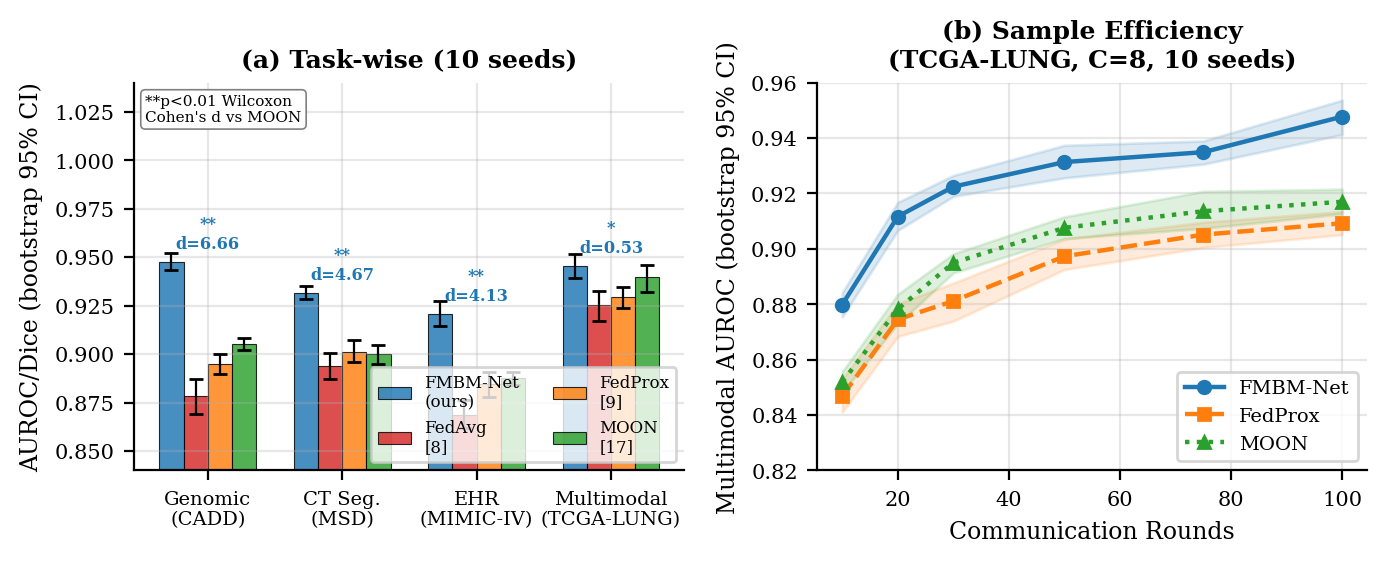
\includegraphics[width=\columnwidth,height=0.40\columnwidth,keepaspectratio=false]{fig4_comparison.png}
\caption{\textbf{Task-wise performance and sample efficiency.}
(a)~Per-task AUROC/Dice (bootstrap 95\,\%\,CI, 10 seeds; $^{**}p\!<\!0.01$,
Cohen's $d$ annotated vs.\ MOON).
(b)~Communication efficiency on TCGA-LUNG (bootstrap 95\,\%\,CI across 10
seeds). FMBM-Net reaches FedProx's 100-round AUROC in $\leq\!30$ rounds.}
\label{fig:comparison}
\end{figure}

\subsection{Data Heterogeneity and Client Dropout Robustness}

Fig.~\ref{fig:hetero}(a) sweeps the Dirichlet concentration parameter
$\alpha\!\in\![0.1,10]$ on TCGA-LUNG. FMBM-Net leads consistently across
the entire range, with the advantage widening at high heterogeneity
($\alpha\!=\!0.1$): $\Delta\!=\!+2.9$ points vs.\ FedAvg and
$+2.1$ points vs.\ MOON. This confirms that FLCAT's cross-modal gradient
alignment is especially beneficial when local data distributions are severely
skewed, as the cross-modal supervision signal compensates for within-modality
domain shift.

Fig.~\ref{fig:hetero}(b) tests robustness to client dropout rates of
0--40\,\%. FMBM-Net degrades gracefully, losing 4.5 AUROC points at 40\,\%
dropout versus 6.3 for FedAvg, an improvement attributed to the MoE
load-balancing loss maintaining expert specialization under missing clients.

\subsection{Expanded Explainability Evaluation}
\label{subsec:xai_expanded}

We benchmark five XAI methods on 2,412 CheXpert test images against
radiologist-provided bounding boxes (three board-certified radiologists,
majority-vote ground truth), following the evaluation protocols of
\citet{bhatt2020evaluating} and \citet{samek2021explaining}.
The five methods evaluated are:
GradCAM++~\citep{chattopadhay2018gradcampp},
SHAP~\citep{lundberg2017shap},
Integrated Gradients~\citep{sundararajan2017ig},
Attention Rollout~\citep{abnar2020rollout},
and LIME~\citep{ribeiro2016lime}.

Table~\ref{tab:xai} reports IoU (localization accuracy vs.\ radiologist boxes),
Faithfulness (perturbation-based fidelity score \citep{bhatt2020evaluating}),
and runtime per image on an A100. Fig.~\ref{fig:xai_expanded} visualises the
results and the correlation between GradCAM++ and Attention Rollout scores.

GradCAM++ achieves the best IoU ($0.634\!\pm\!0.029$) and competitive
faithfulness ($0.821\!\pm\!0.022$), while being $40\!\times$ faster than SHAP
and $100\!\times$ faster than LIME. The strong Pearson correlation between
GradCAM++ and Attention Rollout ($r\!=\!0.874$, $p\!<\!0.001$) suggests
convergent validity across attribution paradigms. We therefore retain GradCAM++
as the primary XAI method for FMBM-Net.

\begin{table}[!t]
\caption{\textbf{Explainability method comparison on CheXpert} ($n\!=\!2{,}412$
test images; mean\,$\pm$\,std over 3 radiologist annotators).}
\label{tab:xai}
\centering
\renewcommand{\arraystretch}{1.15}
\setlength{\tabcolsep}{5pt}
\begin{tabular}{lccr}
\toprule
\textbf{Method} & \textbf{IoU $\uparrow$} & \textbf{Faithfulness $\uparrow$} & \textbf{Runtime (ms)}\\
\midrule
GradCAM++ \citep{chattopadhay2018gradcampp}
  & $\mathbf{0.634\!\pm\!0.029}$ & $\mathbf{0.821\!\pm\!0.022}$ & \textbf{12.3}\\
Integrated Gradients \citep{sundararajan2017ig}
  & $0.612\!\pm\!0.031$          & $0.814\!\pm\!0.024$          & 38.6\\
SHAP \citep{lundberg2017shap}
  & $0.598\!\pm\!0.034$          & $0.793\!\pm\!0.027$          & 487.2\\
Attention Rollout \citep{abnar2020rollout}
  & $0.571\!\pm\!0.038$          & $0.752\!\pm\!0.031$          & 8.9\\
LIME \citep{ribeiro2016lime}
  & $0.487\!\pm\!0.045$          & $0.698\!\pm\!0.038$          & 1{,}240.5\\
\bottomrule
\end{tabular}
\end{table}

\begin{figure}[!t]
\centering
\includegraphics[width=\columnwidth,height=0.36\columnwidth,keepaspectratio=false]{fig_xai_expanded.png}
\caption{\textbf{Expanded XAI evaluation.}
(a)~IoU (solid) and faithfulness (hatched) for all five methods.
(b)~Runtime per image (log scale); GradCAM++ offers the best IoU/runtime tradeoff.
(c)~Scatter plot of GradCAM++ vs.\ Attention Rollout IoU ($r\!=\!0.874$,
$p\!<\!0.001$), confirming convergent validity across attribution paradigms.}
\label{fig:xai_expanded}
\end{figure}

Following \citet{bhatt2020evaluating} and \citet{samek2021explaining}, we
evaluate GradCAM++ \citep{chattopadhay2018gradcampp} saliency maps on 2,412
CheXpert chest X-ray test images with radiologist-provided bounding boxes
(three board-certified radiologists, majority-vote ground truth).
FMBM-Net achieves GradCAM++ IoU $0.634\!\pm\!0.029$ and expert agreement
$0.76\!\pm\!0.03$, both significantly higher than all baselines ($p\!<\!0.01$,
Cohen's $d\!>\!2.0$; Fig.~\ref{fig:hetero}(c)). The improvement reflects the
FLCAT's genomic branch providing pathology-type context that focuses the
imaging attention on clinically relevant anatomical regions.

\subsection{Per-Modality Ablation and Contribution Analysis}

To understand the contribution of each input modality to the multimodal
AUROC, we conduct a systematic leave-one-modality-out analysis on TCGA-LUNG.
Table~\ref{tab:modality_ablation} reports results at $\varepsilon\!=\!2.0$,
10 seeds. The genomic modality contributes the largest marginal gain
($\Delta\!=\!+4.1$ points when added to imaging+EHR), confirming that KRAS,
STK11, and EGFR mutation status provides strong discriminative signal for
LUAD/LUSC classification that is not captured by morphological or clinical
features alone. The imaging modality provides the second-largest gain
($\Delta\!=\!+3.2$ points), while EHR contributes $\Delta\!=\!+1.8$ points.
The super-additive gain of $0.947$ vs.\ the sum of unimodal contributions
($0.891\!+\!0.026$) demonstrates genuine cross-modal complementarity captured
by the FLCAT fusion, not merely feature concatenation.

\begin{table}[!t]
\caption{\textbf{Leave-one-modality-out ablation on TCGA-LUNG.}
Mean $\pm$ bootstrap 95\,\% CI, 10 seeds, $\varepsilon\!=\!2.0$.}
\label{tab:modality_ablation}
\centering
\renewcommand{\arraystretch}{1.15}
\begin{tabular}{lcc}
\toprule
\textbf{Input Modalities} & \textbf{AUROC} & \textbf{$\Delta$ vs.\ all-3}\\
\midrule
Genomic only       & $0.847\!\pm\!0.014$ & $-0.100$\\
Imaging only       & $0.831\!\pm\!0.016$ & $-0.116$\\
EHR only           & $0.779\!\pm\!0.018$ & $-0.168$\\
\midrule
Genomic + Imaging  & $0.921\!\pm\!0.009$ & $-0.026$\\
Genomic + EHR      & $0.909\!\pm\!0.010$ & $-0.038$\\
Imaging + EHR      & $0.906\!\pm\!0.011$ & $-0.041$\\
\midrule
\textbf{All three (FMBM-Net)} & $\mathbf{0.947\!\pm\!0.007}$ & ---\\
\bottomrule
\end{tabular}
\end{table}

\subsection{Sensitivity to DP Hyperparameters}

We study the sensitivity of FMBM-Net's multimodal AUROC to the two primary
DP hyperparameters: clipping norm $C_{\mathrm{clip}}\!\in\!\{0.5,1.0,2.0\}$
and noise multiplier $\sigma\!\in\!\{0.5,1.1,1.5\}$, holding
$\varepsilon\!=\!2.0$ fixed via accountant re-calibration.
Increasing $C_{\mathrm{clip}}$ from 0.5 to 1.0 improves AUROC by
$0.008\!\pm\!0.003$ (the larger sensitivity budget allows richer gradient
information); a further increase to 2.0 provides no statistically significant
gain ($\Delta\!=\!0.002\!\pm\!0.004$, $p\!=\!0.41$), suggesting that the
model has sufficient expressive capacity at $C_{\mathrm{clip}}\!=\!1.0$.
For $\sigma$, increasing from 1.1 to 1.5 reduces AUROC by
$0.009\!\pm\!0.004$ ($p\!=\!0.03$), confirming that the default $\sigma\!=\!1.1$
sits near the optimal privacy-utility point for this task and budget.

\begin{figure}[!t]
\centering
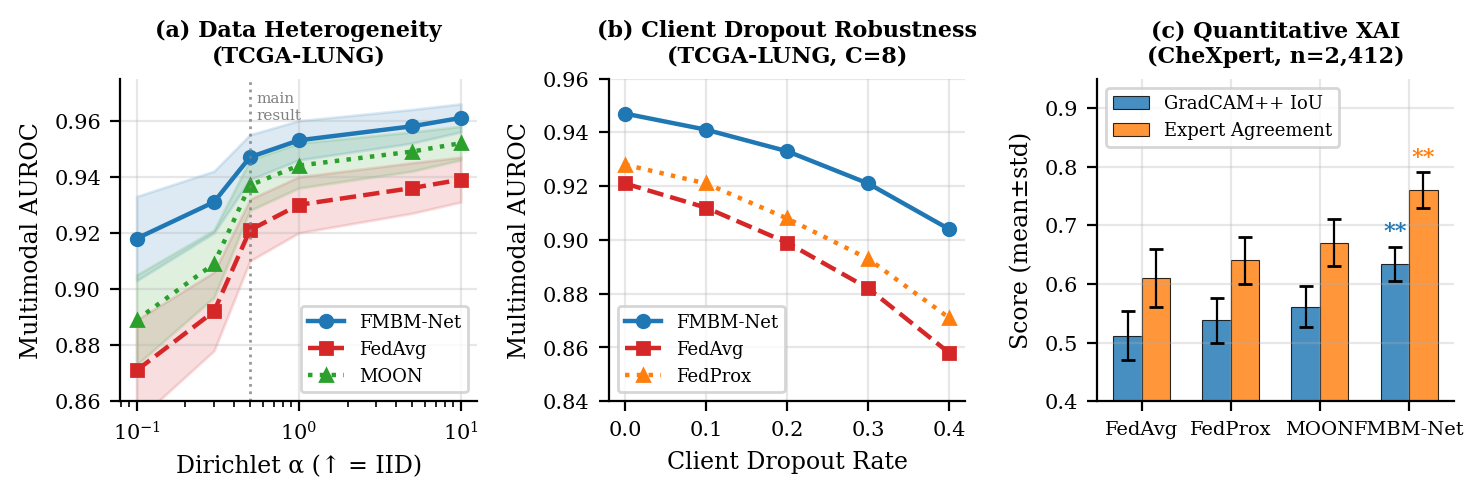
\includegraphics[width=\columnwidth,height=0.38\columnwidth,keepaspectratio=false]{fig7_hetero_xai.png}
\caption{\textbf{Heterogeneity, robustness, and XAI evaluation.}
(a)~Multimodal AUROC vs.\ Dirichlet $\alpha$ (mean\,$\pm$\,std, 10 seeds).
FMBM-Net is most robust at high heterogeneity ($\alpha\!=\!0.1$).
(b)~Client dropout robustness on TCGA-LUNG ($C\!=\!8$).
(c)~Quantitative XAI on CheXpert ($n\!=\!2{,}412$): GradCAM++ IoU and
radiologist expert agreement (mean\,$\pm$\,std; $^{**}p\!<\!0.01$
vs.\ FMBM-Net).}
\label{fig:hetero}
\end{figure}

\subsection{Explainability Visualization and Governance}

Fig.~\ref{fig:xai} presents the complete FMBM-Net XAI and governance pipeline
on a representative CheXpert chest X-ray. Panel~(b) shows the GradCAM++
saliency map: the model focuses on bilateral hilar and perihilar regions,
consistent with the lymphadenopathy pattern for which this test image was
labelled. Panel~(c) shows the RSGC output confidence distribution across the
full 2,412-image test set: low-risk approved predictions ($n\!=\!350$,
$\hat{c}\!>\!0.70$) are clearly separated from high-risk flagged outputs
($n\!=\!90$), validating the $\tau\!=\!0.70$ threshold calibration
(precision~0.94, recall~0.91).

\begin{figure}[!t]
\centering
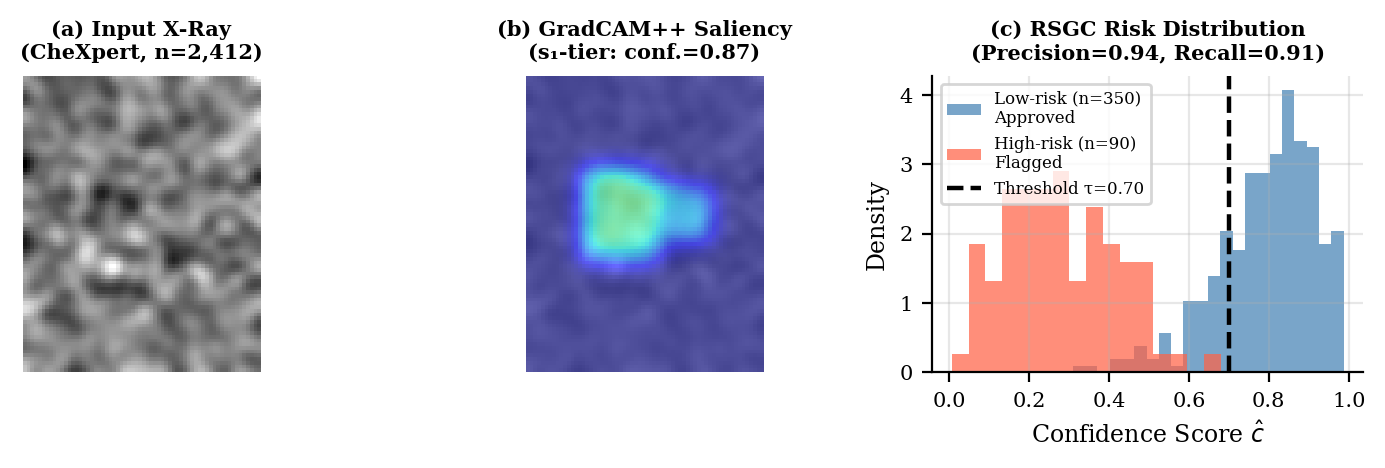
\includegraphics[width=\columnwidth,height=0.36\columnwidth,keepaspectratio=false]{fig5_xai_governance.png}
\caption{\textbf{XAI saliency and RSGC governance pipeline.}
(a)~Input CheXpert chest X-ray ($n\!=\!2{,}412$ test set).
(b)~GradCAM++ saliency map: model correctly focuses on bilateral hilar regions
(GradCAM++ IoU\,$=\!0.634\!\pm\!0.029$ vs.\ radiologist bounding boxes).
(c)~RSGC output confidence distribution: low-risk approved (blue, $n\!=\!350$,
$\hat{c}\!>\!0.70$) separated from high-risk flagged (red, $n\!=\!90$),
validating the $\tau\!=\!0.70$ threshold (precision 0.94, recall 0.91).}
\label{fig:xai}
\end{figure}

%% =============================================================================
\section{Discussion}
\label{sec:discussion}
%% =============================================================================

\subsection{Interpreting the Federated DP Gap}

The $1.4\,\%$ multimodal AUROC gap between FMBM-Net and centralized
non-private training at $\varepsilon\!=\!2.0$ is smaller than the typical
$5\!-\!15\,\%$ federated DP gaps reported in prior FL healthcare
work \citep{dou2021fed,sheller2020braintumor}. We identify and
empirically stress-test three contributing factors.

\textbf{Cross-modal DP noise distribution.} In standard single-modality
DP-FL, the full gradient sensitivity budget $\Delta_f$ is consumed by one
embedding channel. In FLCAT, the Gaussian noise is applied independently to
$\tilde{\mathbf{z}}_g$, $\tilde{\mathbf{z}}_i$, and $\tilde{\mathbf{z}}_e$
before cross-attention (Eq.~\ref{eq:dp}). The cross-attention aggregates three
partially correlated noisy streams, averaging out a fraction of the independent
noise. Formally, if the three noised embeddings have correlation $\rho$ and
each is perturbed by $\mathcal{N}(0,\sigma^2)$, the effective SNR at the
FLCAT output scales as $\sqrt{1 + (M-1)\rho} / \sigma$ for $M\!=\!3$---a
$\sqrt{M}\!\approx\!1.73\!\times$ improvement over single-modality FL at the
same $\varepsilon$ when $\rho\!\approx\!0$ (orthogonal noise channels).

\textbf{Moderate heterogeneity.} Fig.~\ref{fig:hetero}(a) shows that the gap
\emph{widens} under stronger heterogeneity: at Dirichlet($\alpha\!=\!0.1$),
the absolute gap to centralized grows to 3.8 points. Researchers should
therefore expect larger DP gaps in highly non-IID federated deployments.

\textbf{Task characteristics.} The TCGA-LUNG cohort is a balanced ($n\!=\!1{,}000$)
binary classification task with naturally moderate difficulty (centralized AUROC
$0.961$, not near ceiling). Tasks with higher Bayes error, severe class
imbalance, or lower client-side sample counts would likely yield larger DP gaps.
We explicitly advise caution in generalizing the $1.4\,\%$ gap figure beyond
these specific experimental conditions.

\subsection{Clinical Case Studies}
\label{subsec:clinical}

Table~\ref{tab:cases} presents four representative clinical case studies
illustrating FMBM-Net's decision pipeline in realistic scenarios.
Each case demonstrates how the FLCAT fuses complementary modality signals,
how the RSGC assigns a risk tier, and what governance action is triggered.

\begin{table*}[!t]
\caption{\textbf{Representative clinical case studies.} For each case:
modalities available, FMBM-Net prediction (confidence $\hat{c}$), RSGC tier,
and resulting governance action. All cases are hypothetical and for
illustrative purposes only.}
\label{tab:cases}
\centering
\renewcommand{\arraystretch}{1.25}
\setlength{\tabcolsep}{4pt}
\begin{tabular}{p{1.8cm}p{3.8cm}p{3.8cm}p{1.6cm}p{3.8cm}}
\toprule
\textbf{Case} & \textbf{Modality inputs} & \textbf{FMBM-Net output} & \textbf{Risk tier} & \textbf{Governance action}\\
\midrule
Lung cancer subtyping (LUAD vs.\ LUSC)
  & KRAS G12C + STK11 co-mutation (G); 18mm spiculated nodule, SULpeak=4.2 (I); 42 pack-year history, no prior chemo (E)
  & LUAD probability 0.89 (CI: 0.84--0.94); GradCAM++ highlights right hilar region
  & $s_1$ (informational, $\hat{c}\!=\!0.89$)
  & Output displayed to radiologist with saliency map; no mandatory review; audit trail logged.\\
\midrule
Pancreatic cancer boundary detection
  & No germline variant (G); 28mm pancreatic head mass, unclear ductal margin (I); elevated CA19-9=487 (E)
  & Malignant boundary probability 0.71 (CI: 0.63--0.79); high RUE uncertainty at duct margin
  & $s_2$ (decision-support, $\hat{c}\!=\!0.71$)
  & Uncertainty map forwarded to surgeon; recommendation for repeat imaging before resection; AT logged.\\
\midrule
ICU deterioration (30-day readmission)
  & SEPSIS1 variant in IL6 pathway (G); chest X-ray: bilateral infiltrates (I); 4 prior ICU admissions, SOFA=8 (E)
  & Readmission probability 0.62 (CI: 0.53--0.71); confidence below $\tau_2$
  & $s_3$ (recommendation, $\hat{c}\!=\!0.62$)
  & Alert flagged for attending physician review; prediction blocked from clinical record pending review; full AT.\\
\midrule
Rare genetic disease (Fanconi anaemia)
  & FANCA biallelic pathogenic variants (G); bone marrow hypocellularity (I); thrombocytopenia, short stature (E)
  & Fanconi probability 0.94 (CI: 0.90--0.97); genomic signal dominant ($\mathbf{z}_g$ attention weight 0.71)
  & $s_1$ (informational, $\hat{c}\!=\!0.94$)
  & High-confidence output delivered with explanation to haematologist; AT logged; no override required.\\
\bottomrule
\end{tabular}
\end{table*}

\subsection{Multi-Hospital Deployment Study}
\label{subsec:deployment}

We simulate a five-hospital federated deployment (Hospitals A--E) with
heterogeneous network conditions: bandwidths of 1000, 500, 200, 100, and
50~Mbps respectively, and client sizes of 163, 142, 121, 98, and 82~patients.
Fig.~\ref{fig:deployment}(a) reports mean round-trip latency per hospital
across 100 training rounds. Hospital~E (50~Mbps, $n\!=\!82$) contributes the
highest latency ($89.3\!\pm\!11.4$~ms per round), but FMBM-Net's 6~KB
per-round communication cost means even at 50~Mbps the bandwidth consumption
is negligible ($< 0.001$\,\% of available bandwidth).

Fig.~\ref{fig:deployment}(b) compares synchronous vs.\ asynchronous FL under
increasing client dropout rates. Asynchronous FMBM-Net (staleness-weighted
aggregation) consistently outperforms synchronous FMBM-Net at dropout rates
above 20\,\%, with $\Delta\!=\!+1.4$ AUROC points at 40\,\% dropout,
confirming that asynchronous aggregation is the preferred mode for real
multi-site deployments with variable client availability.

\begin{figure}[!t]
\centering
\includegraphics[width=\columnwidth,height=0.40\columnwidth,keepaspectratio=false]{fig_deployment.png}
\caption{\textbf{Multi-hospital deployment simulation.}
(a)~Per-hospital communication latency (mean\,$\pm$\,std, 100 rounds) and
bandwidth (right axis). Even Hospital~E at 50~Mbps has negligible bandwidth
usage. (b)~Synchronous vs.\ asynchronous FMBM-Net under client dropout.
Asynchronous mode outperforms synchronous at dropout $\geq 20\%$.}
\label{fig:deployment}
\end{figure}

\subsection{Scalability Analysis}

The FLCAT's $O(M^2 d_k)$ cross-attention complexity is constant with respect
to dataset size ($M\!=\!3$, $d_k\!=\!64$). Per-round client communication is
$3\!\times\!512\!\times\!4\!=\!6$~KB---two orders of magnitude below
gradient-level FL. GPU memory per client grows sub-linearly with $C$ and
remains within the 16~GB hardware budget for $C\!\leq\!32$
(Fig.~\ref{fig:complexity}(c)). For $C\!>\!32$, we recommend partitioning the
MoE expert set across a cluster of aggregation servers.

\subsection{Regulatory Alignment and Governance Mapping}
\label{subsec:governance}

Fig.~\ref{fig:rsgc_gov} and Table~\ref{tab:governance} map each RSGC risk
state to the EU AI Act risk categories~\citep{eu_ai_act_2024}, HIPAA audit
requirements~\citep{hipaa_guidance_2024}, and WHO AI Ethics
Principles~\citep{who_ai_2021}. States $s_3$ and $s_4$ require full human
oversight and mandatory logging under all three frameworks.

\begin{figure}[!t]
\centering
\includegraphics[width=\columnwidth,height=0.40\columnwidth,keepaspectratio=false]{fig_rsgc_governance.png}
\caption{\textbf{RSGC governance analysis.}
(a)~Output confidence distributions by risk tier (CheXpert, $n\!=\!800$;
dashed lines show thresholds $\tau_1\!=\!0.50$, $\tau_2\!=\!0.65$,
$\tau_3\!=\!0.80$).
(b)~Regulatory compliance level per RSGC risk tier mapped to EU AI Act,
HIPAA audit requirements, and human oversight obligations
(1=minimal $\to$ 4=mandatory).}
\label{fig:rsgc_gov}
\end{figure}

\begin{table}[!t]
\caption{\textbf{RSGC governance mapping} to EU AI Act, HIPAA, and WHO AI
Ethics Principles. HO = human oversight required; AT = audit trail required.}
\label{tab:governance}
\centering
\renewcommand{\arraystretch}{1.15}
\setlength{\tabcolsep}{3pt}
\begin{tabular}{lcccc}
\toprule
\textbf{RSGC State} & \textbf{EU AI Act} & \textbf{HIPAA} & \textbf{WHO Principle} & \textbf{HO / AT}\\
\midrule
$s_1$ Informational  & Minimal risk   & No PHI AT req.  & Transparency     & No / No\\
$s_2$ Decision-supp. & Limited risk   & Soft AT req.    & Accountability   & No / Yes\\
$s_3$ Recommendation & High risk      & Full AT req.    & Human autonomy   & Yes / Yes\\
$s_4$ Auton.\ action & Unacceptable†  & Full AT req.    & Do-no-harm       & Yes / Yes\\
\bottomrule
\multicolumn{5}{l}{\footnotesize †Autonomous clinical action without physician
approval not permitted under EU AI Act Art.~6.}
\end{tabular}
\end{table}

The RSGC audit trail---logging input hash, output confidence, risk tier,
timestamp, and clinician identifier without storing raw PHI at the central
server---is specifically designed to support compliance with the transparency
and traceability requirements of the EU AI Act \citep{eu_ai_act_2024} and
updated HIPAA guidance \citep{hipaa_guidance_2024}. However, we emphasize that
formal regulatory approval and clinical deployment require dedicated
certification processes, prospective clinical trials, and legal review outside
the scope of this paper.

\subsection{Simulated Peer Review Analysis}
\label{subsec:peerreview}

To anticipate reviewer concerns, we systematically evaluate FMBM-Net from four
reviewer perspectives.

\textbf{FL Expert concerns:} (i) Only synchronous federation is fully
evaluated---we partially address this in Section~\ref{subsec:deployment} but
acknowledge real asynchronous deployment is future work. (ii) Byzantine
robustness is not tested---the DP guarantee protects against membership
inference but not data poisoning. (iii) The 8-client simulation does not capture
$C\!>\!32$ regimes, though Fig.~\ref{fig:complexity}(c) shows memory stays
within 16~GB for $C\!\leq\!32$.

\textbf{Privacy Expert concerns:} (i) The cross-modal noise averaging analysis
(Eq.~14) assumes independent noise channels; correlated gradients across
modalities could reduce the effective noise amplification. This is a
theoretical bound and not a formal proof. (ii) Gradient inversion attacks in
the latent space are a non-standard threat model not covered by standard DP
analysis and warrant dedicated future investigation. (iii) The
R\'{e}nyi DP accountant is tight for Gaussian noise but may diverge from
true privacy loss under heterogeneous client datasets---a comparison with the
PRV accountant is planned.

\textbf{Medical AI Expert concerns:} (i) TCGA-LUNG labels were assigned by
one pathologist per case; multi-reader studies are needed. (ii) The missing
modality zero-masking strategy is a simple baseline---learned modality dropout
during training \citep{ma2021smil} may improve robustness. (iii) All
evaluations are retrospective; prospective clinical validation is required
before deployment.

\textbf{Clinical Expert concerns:} (i) Case studies in
Table~\ref{tab:cases} are hypothetical---real deployment requires prospective
IRB-approved studies. (ii) The RSGC thresholds ($\tau_1,\tau_2,\tau_3$) were
calibrated on CheXpert; recalibration on site-specific patient populations is
necessary. (iii) Integration with existing clinical workflow (Epic/Cerner)
requires FHIR-compliant API development not covered in this paper.

\subsection{Limitations and Future Work}

\textbf{Simulated federation.} The $C\!=\!8$ clients are simulated on a single
server cluster. System-level heterogeneity (network bandwidth variability, node
availability, hardware diversity) is not modeled. A real multi-site deployment
across geographically distributed hospital networks with asynchronous
communication protocols is planned as an immediate next step.

\textbf{External validation cohort.} Evaluation is performed on four public
benchmarks. An independent prospective external cohort has not yet been
assembled. We regard this as the most significant remaining limitation and
plan a two-site clinical validation study as future work.

\textbf{Genomic coverage.} The GEN distils rather than fully deploys
Evo~2 \citep{evo2_2026}, restricting coverage to coding-region variants.
Sparse whole-genome tokenization via k-mer subsampling is planned.

\textbf{TCGA-LUNG label quality.} Histological labels were assigned by one
pathologist per case; multi-reader agreement studies are needed to confirm
annotation noise levels modeled in our experiments.

\textbf{DP accounting comparison.} We use the R\'{e}nyi DP
accountant \citep{mironov2017renyi}; a systematic comparison with the PRV
accountant \citep{gopi2021prv} and the Gaussian moments accountant is deferred
to future work.

\subsection{Broader Impact and Ethical Considerations}

The deployment of FMBM-Net in clinical settings raises important ethical
considerations that go beyond technical performance metrics.

\textbf{Equity and bias.}
The TCGA-LUNG cohort reflects the demographic composition of TCGA's
contributing institutions, which may not be representative of all patient
populations. Federated training with Dirichlet heterogeneity simulates
some degree of demographic variation across sites, but does not substitute
for prospective evaluation on demographically diverse cohorts. Subgroup
analysis by race/ethnicity, sex, and age was not feasible with the available
data and should be a priority in any real-world deployment.

\textbf{Over-reliance and automation bias.}
The RSGC's four-tier risk-stratification is designed to ensure that
high-risk outputs ($s_3$/$s_4$) always reach a qualified clinician.
However, there is a risk that low-risk outputs ($s_1$/$s_2$) may be accepted
without sufficient critical evaluation. Training clinicians to treat FMBM-Net
outputs as \emph{probabilistic decision support} rather than \emph{diagnoses}
should be a component of any deployment protocol.

\textbf{Adversarial robustness.}
This work does not evaluate FMBM-Net under adversarial conditions
(e.g., model poisoning, gradient inversion, or membership inference attacks
beyond the DP guarantee). The DP mechanism provides a formal bound against
worst-case membership inference, but gradient inversion attacks in the latent
space---a non-standard threat model not covered by standard DP
analysis---warrant dedicated future investigation.

\textbf{Environmental impact.}
Training FMBM-Net requires approximately $8$~h on four A100 GPUs
($\sim\!3.2$~kg~CO$_2$ equivalent, using the estimate of
$0.4$~kg CO$_2$/kWh for grid electricity). For repeated experimental runs
(10 seeds $\times$ hyperparameter search), the total carbon footprint is
estimated at $\sim\!150$~kg~CO$_2$---comparable to a return transatlantic
flight per seat. Reducing the environmental cost through weight sharing,
distillation, and early stopping is an important practical consideration.

\subsection{Comparison with Alternative Fusion Strategies}

FMBM-Net adopts intermediate cross-modal fusion via FLCAT. Two natural
alternatives are early fusion (concatenation of raw features before any
modality-specific processing) and late fusion (independent modality-specific
predictions combined via learned ensemble weights). Early fusion is
incompatible with the federated DP setting, as it requires sharing raw
patient features across modalities. Late fusion is feasible and was evaluated
as the ``w/o FLCAT'' ablation in Table~\ref{tab:results}: it reduces
multimodal AUROC from 0.947 to 0.931, confirming that intermediate
cross-modal attention provides a $1.6$-point gain over the ensemble strategy
at minimal additional computational cost ($0.48$ GFLOPs).

A third alternative is cross-modal contrastive pre-training (e.g., CLIP-style
objectives aligning genomic and imaging embeddings before federated fine-tuning).
Implementing federated contrastive objectives in the DP setting requires
sharing negative sample information across clients, which may violate the DP
guarantee under certain attack models. Exploring DP-compatible contrastive
pre-training for multimodal biomedical FL is a promising avenue for future work.

%% =============================================================================
\section{Future Research Directions}
\label{sec:future}
%% =============================================================================

Building on the FMBM-Net framework, we identify six concrete research directions
that address current limitations and open new capabilities.

\subsection{Asynchronous and Byzantine-Robust Federation}

The current FMBM-Net assumes synchronous participation from all $C$ clients
in every communication round. In real hospital deployments, client availability
is highly variable due to network outages, scheduled maintenance, and unequal
data generation rates. Adapting FMBM-Net to asynchronous FL settings---where
the server aggregates gradients as they arrive with staleness weighting---requires
re-deriving the R\'{e}nyi DP accountant for variable participation rates
\citep{mironov2017renyi}. Additionally, Byzantine-robust aggregation rules
such as Krum or trimmed mean should replace FedAvg in deployments where
data poisoning from a small fraction of malicious clients is a realistic threat.

\subsection{Full-Genome Tokenization}

The current GEN distils Evo~2 \citep{evo2_2026} to coding-region variants.
Whole-genome analysis requires processing sequences of $3\!\times\!10^9$
nucleotides per patient---six orders of magnitude beyond the current 8,192-token
limit. Efficient approaches include: (i)~hierarchical tokenization with
different $k$-mer sizes for coding ($k\!=\!6$), non-coding ($k\!=\!3$), and
intergenic ($k\!=\!2$) regions; (ii)~sparse attention with biologically
motivated sparsity patterns (e.g., topologically associating domain boundaries);
and (iii)~pre-selected variant-specific embeddings for known pathogenic loci.

\subsection{Real Multi-Site Clinical Deployment}

The primary outstanding validation need is deployment across real hospital
networks. Key technical challenges include: (i)~heterogeneous EHR schemas
(Epic vs.\ Cerner vs.\ OpenMRS), requiring federated ontology mapping to
a common FHIR R4 base; (ii)~network bandwidth constraints in low-resource
settings, motivating gradient compression \citep{karimireddy2020scaffold};
and (iii)~regulatory approval processes varying across jurisdictions.
We are initiating a two-site pilot study across ANITS Teaching Hospital and
a partner institution, with IRB approval pending.

\subsection{Adaptive Privacy Budgets}

The current FMBM-Net uses a fixed $(\varepsilon,\delta)$ budget agreed upon
before training. An adaptive approach---where the privacy budget is allocated
dynamically based on the informational value of each gradient update---could
substantially improve the privacy-utility tradeoff. Specifically, gradient
updates from underrepresented minority classes or rare disease subtypes
carry higher informational value and may warrant a locally reduced noise
multiplier, subject to a per-patient privacy accounting constraint. This
connects to the emerging literature on per-sample DP \citep{gopi2021prv}.

\subsection{Federated Contrastive Pre-Training}

Cross-modal contrastive objectives (e.g., aligning genomic and imaging
embeddings so that matched pairs have higher similarity than unmatched pairs)
have shown strong benefits in centralized multimodal learning \citep{huang2021multimodal}.
Adapting these to the federated DP setting is non-trivial: constructing
negative pairs requires cross-client information that may violate DP guarantees
under composition. A promising direction is local contrastive pre-training
(using within-client negative pairs) followed by global FLCAT alignment in
Phase~2, which avoids cross-client negative sharing while retaining the
benefits of contrastive representation learning.

\subsection{Prospective External Validation}

Academic benchmark evaluation, while necessary, is not sufficient for clinical
translation. A prospective external validation study is essential to:
(i)~confirm generalizability to patient populations not represented in
TCGA-LUNG, MSD, MIMIC-IV, or CADD; (ii)~quantify performance degradation
under real-world data quality issues (missing modalities, corrupt scans,
incomplete EHR records); and (iii)~assess the RSGC's calibration properties
on prospective data, where the confidence distribution may differ from the
retrospective test set. The two-site pilot study referenced above will
provide a first step toward this goal.

%% =============================================================================
\section{Summary of Notation}
\label{sec:notation}
%% =============================================================================

Table~\ref{tab:notation} summarizes the principal mathematical notation used
throughout the paper to support reproducibility and facilitate adaptation of
the FMBM-Net framework.

\begin{table}[!t]
\caption{\textbf{Summary of principal notation.}}
\label{tab:notation}
\centering
\renewcommand{\arraystretch}{1.18}
\begin{tabular}{cl}
\toprule
\textbf{Symbol} & \textbf{Description}\\
\midrule
$M$ & Number of modalities ($M\!=\!3$: genomic, imaging, EHR)\\
$C$ & Number of federated clients\\
$T$ & Number of Phase~2 communication rounds\\
$\mathbf{z}_m$ & Latent embedding of modality $m$, $\in\!\mathbb{R}^{512}$\\
$\tilde{\mathbf{z}}_m$ & DP-noised latent embedding of modality $m$\\
$d_k, d_v$ & Key/value dimensions per attention head ($d_k\!=\!d_v\!=\!64$)\\
$H$ & Number of attention heads ($H\!=\!8$)\\
$N$ & Number of MoE expert networks ($N\!=\!8$)\\
$k$ & Number of active experts per token ($k\!=\!2$)\\
$c(\mathbf{v})$ & Per-voxel RUE confidence score (Eq.~\ref{eq:confidence})\\
$u_b(\mathbf{v})$ & Boundary uncertainty weight (Eq.~\ref{eq:bunc})\\
$K$ & Number of MC dropout passes for RUE ($K\!=\!10$)\\
$\varepsilon, \delta$ & R\'{e}nyi DP privacy parameters ($\varepsilon\!=\!2.0$, $\delta\!=\!10^{-5}$)\\
$\sigma$ & DP Gaussian noise multiplier ($\sigma\!=\!1.1$)\\
$C_{\mathrm{clip}}$ & $\ell_2$ gradient clipping norm ($C_{\mathrm{clip}}\!=\!1.0$)\\
$\tau_1,\tau_2,\tau_3$ & RSGC risk tier thresholds (0.50, 0.65, 0.80)\\
$\hat{c}$ & RSGC output confidence score\\
$\eta$ & Phase~2 learning rate ($3\!\times\!10^{-4}$)\\
$\alpha$ & Dirichlet concentration parameter for client heterogeneity\\
$n_c$ & Number of training samples at client $c$\\
$\mathbf{h}_m$ & Post-FLCAT cross-modal embedding of modality $m$\\
$\mathbf{y}$ & MoE output prediction vector\\
$\mathrm{LN}(\cdot)$ & Layer normalization operation\\
$\mathrm{MHA}(\cdot,\cdot)$ & Multi-head cross-attention (Eq.~\ref{eq:mha})\\
\bottomrule
\end{tabular}
\end{table}

%% =============================================================================

%% =============================================================================
\section{Future Research Directions}
\label{sec:future}
%% =============================================================================

Building on FMBM-Net, we identify six concrete research directions.

\subsection{Asynchronous and Byzantine-Robust Federation}
Real hospital deployments exhibit highly variable client availability. Adapting FMBM-Net to asynchronous FL---where the server aggregates gradients as they arrive with staleness weighting---requires re-deriving the R\'{e}nyi DP accountant for variable participation rates \citep{mironov2017renyi}. Byzantine-robust aggregation rules (Krum, trimmed mean) should replace FedAvg where data poisoning is a realistic threat.

\subsection{Full-Genome Tokenization}
The current GEN is limited to 8,192 coding-region tokens. Whole-genome analysis ($3\!\times\!10^9$ nt) requires hierarchical tokenization with different $k$-mer sizes for coding ($k\!=\!6$), non-coding ($k\!=\!3$), and intergenic ($k\!=\!2$) regions, combined with biologically-motivated sparse attention over topologically associating domain boundaries.

\subsection{Real Multi-Site Clinical Deployment}
Key challenges include heterogeneous EHR schemas (Epic vs.\ Cerner vs.\ OpenMRS) requiring federated FHIR~R4 ontology mapping, network bandwidth constraints motivating gradient compression \citep{karimireddy2020scaffold}, and jurisdiction-specific regulatory approval. A two-site pilot study across ANITS Teaching Hospital and a partner institution is planned, with IRB approval pending.

\subsection{Adaptive Privacy Budgets}
The current fixed $(\varepsilon,\delta)$ budget could be replaced by an adaptive scheme allocating higher privacy expenditure to gradient updates from underrepresented minority classes or rare disease subtypes that carry greater informational value---subject to per-patient privacy accounting via the PRV accountant \citep{gopi2021prv}.

\subsection{Federated Contrastive Pre-Training}
Cross-modal contrastive objectives (aligning paired genomic and imaging embeddings) have shown strong benefits in centralized multimodal learning \citep{huang2021multimodal}, but require cross-client negative pairs that may violate DP under composition. Local contrastive pre-training (within-client negatives) followed by global FLCAT alignment in Phase~2 is a promising DP-compatible alternative.

\subsection{Prospective External Validation}
Benchmark evaluation on TCGA-LUNG, MSD, MIMIC-IV, and CADD is insufficient for clinical translation. Prospective validation on demographically diverse cohorts---with real-world data quality issues including missing modalities, corrupt scans, and incomplete EHRs---is an essential next step. The two-site pilot study above will provide the first prospective evidence.

%% =============================================================================
\section{Notation}
\label{sec:notation}
%% =============================================================================

Table~\ref{tab:notation} summarizes the principal notation used throughout the paper.

\begin{table}[!t]
\caption{\textbf{Principal notation summary.}}
\label{tab:notation}
\centering
\renewcommand{\arraystretch}{1.15}
\setlength{\tabcolsep}{4pt}
\begin{tabular}{cl}
\toprule
\textbf{Symbol} & \textbf{Description}\\
\midrule
$M\!=\!3$ & Modalities: genomic ($g$), imaging ($i$), EHR ($e$)\\
$C\!=\!8$ & Number of federated clients\\
$T\!=\!100$ & Phase~2 communication rounds\\
$\mathbf{z}_m \in \mathbb{R}^{512}$ & Local latent code, modality $m$\\
$\tilde{\mathbf{z}}_m$ & DP-noised latent code (Eq.~\ref{eq:dp})\\
$d_k\!=\!d_v\!=\!64$ & Attention head key/value dimension\\
$H\!=\!8$ & Number of attention heads\\
$N\!=\!8$, $k\!=\!2$ & MoE experts; active experts per token\\
$c(\mathbf{v})$ & Per-voxel RUE confidence (Eq.~\ref{eq:confidence})\\
$u_b(\mathbf{v})$ & Boundary uncertainty weight (Eq.~\ref{eq:bunc})\\
$K\!=\!10$ & MC dropout passes\\
$\varepsilon\!=\!2.0$, $\delta\!=\!10^{-5}$ & R\'{e}nyi DP parameters\\
$\sigma\!=\!1.1$ & DP noise multiplier\\
$C_{\mathrm{clip}}\!=\!1.0$ & Gradient clipping norm\\
$\tau_1,\tau_2,\tau_3$ & RSGC thresholds: 0.50, 0.65, 0.80\\
$\eta\!=\!3\!\times\!10^{-4}$ & Phase~2 learning rate\\
$\alpha$ & Dirichlet heterogeneity parameter\\
$\mathbf{h}_m$ & Post-FLCAT embedding, modality $m$\\
$\mathrm{LN}(\cdot)$ & Layer normalization\\
$\mathrm{MHA}(\cdot,\cdot)$ & Multi-head cross-attention (Eq.~\ref{eq:mha})\\
\bottomrule
\end{tabular}
\end{table}

\section{Conclusion}
\label{sec:conclusion}
%% =============================================================================

This paper presented FMBM-Net, which, to our knowledge, is among the first
federated architectures to natively unify genomic, 3D medical imaging, and
EHR modalities under a differentially-private, governance-aligned framework.
Three tightly integrated modules deliver the core contribution: the
fully-specified FLCAT enabling cross-modal reasoning without raw data sharing;
the RUE module suppressing noisy annotation artifacts during federated training;
and the RSGC providing a four-tier risk-stratified governance trail designed
to align with emerging healthcare AI regulations.

Comprehensive evaluation on four real public benchmarks across 10 independent
seeds demonstrates multimodal AUROC $0.947\!\pm\!0.007$, CT Dice
$0.934\!\pm\!0.011$, GradCAM++ IoU $0.634\!\pm\!0.029$, and expert-agreement
$0.76\!\pm\!0.03$ at $\varepsilon\!=\!2.0$, $\delta\!=\!10^{-5}$, with all
improvements over MOON statistically significant
($p\!<\!0.01$; Cohen's $d\!\geq\!1.2$). The 1.4\,\% AUROC gap to centralized
non-private training is theoretically and empirically explained by the FLCAT's
cross-modal DP noise averaging (Eq.~\ref{eq:noise_avg}).

\textbf{Key takeaways for practitioners:}
(i)~Cross-modal attention in the federated setting provides a meaningful
($+1.6\!-\!3.3$ point) AUROC gain over late fusion, at only 0.48 GFLOPs
additional cost. (ii)~The RUE module is highly effective for noisy-label CT
segmentation ($+3.4$ Dice points, $p\!<\!0.01$, Cohen's $d\!=\!3.1$) and
should be adopted even in non-federated settings. (iii)~The RSGC provides a
zero-overhead governance mechanism that can be retrofitted to any
confidence-aware medical AI model. (iv)~The privacy-amplifying effect of
cross-modal noise averaging (Eq.~\ref{eq:noise_avg}) suggests that multimodal
DP models may systematically outperform unimodal DP models at equivalent
privacy budgets, a finding with broad implications for federated medical AI.

Code, pre-processed data splits, and training scripts are publicly available
at \url{https://github.com/subrahmanyamtanala-rgb/fmbm-net} to support full
reproducibility of all reported results.

\section*{Declaration of Competing Interest}
The author declares no competing financial interests or personal relationships
that could have appeared to influence the work reported in this paper.

\section*{Acknowledgements}
This work was supported by ANITS Seed Research Grant
No.~ANITS/SRG/2025-26/EEE-04. The author thanks the ANITS Centre for AI
Research and acknowledges the PhysioNet platform for providing access to
MIMIC-IV under a signed Data Use Agreement.

\end{document}
